% !TEX encoding = UTF-8 Unicode
\documentclass[11pt]{article}

\usepackage[letterpaper, margin=1.5cm]{geometry}
\usepackage{graphicx}
\usepackage[english]{babel}
\usepackage[utf8]{inputenc}
\usepackage{amsmath,amsfonts,amssymb}
\usepackage{hyperref}
\usepackage[square,numbers,sort&compress]{natbib}
\newcommand{\TODO}[1]{\begingroup\color{red}#1\endgroup}
\usepackage{booktabs}
\usepackage{color}
\usepackage{booktabs}
\newcommand{\tabitem}{\llap{}}
\usepackage{adjustbox}
\usepackage{longtable}
\usepackage{footnote}
\makesavenoteenv{tabular}
\makesavenoteenv{table}
\usepackage{footmisc} %reference footnotes
\usepackage{listings}
\usepackage{rotating}

\newcommand{\CAVH}[1]{\begingroup\color{red}#1\endgroup}
\newcommand{\ADD}[1]{\begingroup\color{blue}#1\endgroup}
\begin{document}
\title{A new strategy to characterize the domain architecture structure of 
proteins of the innate inmune system in tunicate species}
% Use \titlerunning{Short Title} for an abbreviated version of
% your contribution title if the original one is too long
\author{Cristian A. Velandia-Huerto*, Ernesto Parra, Federico D. 
Brown, Adriaan Gittenberger, \\ Peter F. Stadler and Clara I. 
Berm\'{u}dez-Santana}

% Use \authorrunning{Short Title} for an abbreviated version of
% your contribution title if the original one is too long
%\date{}

\maketitle

\begin{itemize}
\item \TODO{Include information about D.vexillum sequencing and assembly 
process: Clara and Ernesto.}
\item \TODO{Change everything related with another databases different to Pfam}. 
\item \TODO{Discuss about the biological meaning of the different architecture 
strategies}
\item \TODO{Discuss about the ProteinOrtho strategy to create innane immune 
system groups, based on protein comparison, but grouped by common domain's 
architectures}.
\item \TODO{If yes, what is the best option to detect protein orthologs. Based 
on complete protein? or splitting  by protein domains?}
\item \TODO{Plot: Distribution of architectures? (by specie)}
\item \TODO{Biological meaning of the detected innate immune proteins on 
tunicates.}
\item \TODO{Best way to publish the paper and the new pipeline?}
\end{itemize}


\section{Introduction}

The challenge of having a feasible and fast tool to characterize the sequences 
of many new genomes of non-model organisms has been increasing the need to 
develop strategies that extract the maximum information of the gen architecture. 
This trend has become the last purpose of the gene annotation where given a 
candidate coding sequence its biological function is assigned to further 
functional or evolutionary studies \cite{aken2016ensembl} 
\cite{birney2004overview} \cite{ashburner2000gene} \cite{tatusov2000cog} 
\cite{tatusova2016ncbi}. 

Nevertheless, to annotate, researchers tackle two main computational problems, 
one to detect first on genomic subregions the corresponding coding regions and 
then after or simultaneously assign functionality. Due to the broad complexity 
of the regulation of the eukaryotic gene expression which relies on 
the recognition of alternative motifs of subsequences that ends in alternatives 
transcripts is today more harder the definition of a gene boundary making the 
annotation a more complex task than CDS predictions\cite{yandell2012}. 

At the begining, gene annotation was based on ab initio methods that screened 
for  specific signals  in eukaryotic genes, such as TATA box signals, 
exon/intronic definitions and polyadenylation signals \cite{claverie}. Tools 
like GENSCAN introduced originally a probabilistic model of human gene structure 
\cite{genescan}. Then, in 2005 a great advance in the annotation processes was 
got by the introduction of the tool AUGUSTUS \cite{augustus} which allows quite 
accurately gene prediction and today there are versions that can be trained by 
integrating RNAseq data, short cDNAs etc. AUGUSTUS corresponds to the 
Generalized Hidden Markov Model. Other methods as GeneID uses a rules-based 
heuristic method to assemble the typical signals of genes in a product or model 
more likely. In the post-genomic era, gene annotation pipelines have been 
handled the heterogeneity of the available expression information of ESTs, 
RNA-seq or proteomic data in two main ways: by manual curation as such as the 
VEGA-HAVANA project of the Wellcome Trust Sanger Institute and by using 
automated process or hybrids methods which integrate homologies with coherent 
patterns of known genes of other species to characterize all the functional 
elements that make up the genes, ending with the assignment of a biological 
function to a genomic sequence \cite{aken2016ensembl} \cite{birney2004overview}. 
For the case of vertebrates as well as some tunicate species which are the 
closest relatives to vertebrates \cite{delsuc2006} their genomes have undergone 
a rigorous annotation process widely accepted in comparative genomics of 
vertebrates such as the annotation pipeline of the European molecular biology 
laboratory (EMBL) that integrates the experimental information of 70 vertebrate 
and other metazoan species on the genome browser Ensembl \cite{aken2016ensembl}.

In this work we focused on some species of the sub-phylum Tunicata since are 
key organisms to study the evolution of the immune system due to its 
phylogenetic position on the Tree of Life just before the biological phenomenon 
known as the immunology big-bang that gave rise to the origin of the Adaptive 
Immune System \cite{bernstein1996}. Additionaly, this group is characterized by 
the great diversity of style of life and the world widely distribution in 
ecological niches that might force them to design different immune response to 
survive in their habitats. Since tunicates can live as solitary sessile or 
pelagic or to live in colonies they have complex relationships between the 
environment, so diversity in the composition of gene of the immune system is 
expected  \cite{carroll2008evo, berna2014evolutionary}. 

Nevertheless, the global importance of this group, the genomic studies are 
scarce as the comparative as well. So far, the genomes of three solitary 
ascidians have been annotated: the sessiles \textit{Ciona savignyi} and 
\textit{Ciona intestinalis} mapped on its $14$ chromosomes \cite{dehal2002draft, 
small2007haplome} and the pelagic \textit {Oikopleura dioica} 
\cite{denoeud2010plasticity}, \cite{seo2001miniature}. However, for colonial 
ascidians, only the genome of \textit{Botrillus schlosseri} mapped to $13$ 
chromosomes \cite{voskoboynik2013genome} and recently the detection of ncRNAs in 
the draft genome of the carpet sea squirt \textit{Didemnum vexillum} 
\cite{velandia2016a} are available.  From preliminary comparative genomics 
between some tunicates and genomes of some chordates have been identified 
expansion of gene families by events of local duplications, but also gene loss. 
Some genes conserved between the amphioxus and the human have also been 
identified based on the tunicate genome of \textit{C. intestinalis}. The 
complexity of the genomic organization of those tunicates has led to different 
authors to formulate the idea of the existence in their evolution of processes 
of genomic re-structuring in all or some tunicates genomes 
\cite{putnam2008amphioxus}. In addition, since the rate of evolution of other 
chordates has been constant, it is considered that in the tunicates evolution 
rates are high and therefore specific patterns of organization of all their 
genes are expected \cite{putnam2008amphioxus, berna2014evolutionary}. Based on 
complex events that might shape the variety of tunicate genome structure we 
posit that they might act not only in the evolution of the genome architecture 
but also in the evolution of complex systems like the immune system. To study 
that idea we based first on Paalsson, et al. 2007 who claimed that the immune 
system comes from a few ancestral proteins, selected and fixed throughout the 
evolution and proposed that the entire immune system has been based 
fundamentally from nine ancestral domains which are conserved throughout the 
evolution of multiple organisms \cite{paalsson2007building}. We propose in this 
survey to use protein domains as the most elementary evolutionary module of the 
immune system to built a picture of domain architectures turnover that might 
resemble the effect of evolutionary driving force that led to the complexity of 
the immune system in tunicates. Since domain variability implies new protein 
organizations (without considering that there is also re-ordering of exons), 
then it is extremely interesting to describe if the domain variability would 
have favored the creation of new protein architectures that could be positively 
selected in tunicates\cite{paalsson2007building}. Therefore data used in this 
survey are built on the domains of receptors associated with the innate 
immune system of known canonical architectures. Our alternative  homology 
search is 
proposed to complement the classical homologies searches like BLAST which are 
not very sensitive to traceback homologues relationships among gene with complex 
structures\cite{Buckley64}. In some genes of the inmune system is not rare to 
find copies and reshuffling of domains. In this survey we searched for canonical 
and like-canonical protein domain architecture of the innate immune system genes 
since similar to other invertebrates, tunicates rely only on innate 
immunology\cite{franchi2017}. We designed different comparison strategies for a 
flexible screening of architectures since tandem copies or rearrangement of 
domains have been reported in the evolution of domains in proteins 
\cite{Forslund2012}.

\section*{Methods and Materials}

\subsection*{Protein domain architectures of reference}
We started with annotated and curated genes from \texttt{InnateDB} 
\cite{Breuer01012013} and \texttt{Insect Innate Immunity Database} (IIID) 
\cite{Brucker2012} in order to define a \textsl{gold standard} set of domain 
architectures of proteins of the innate immune system. At \texttt{InnateDB} many 
other immune-specific databases are linked as \texttt{Immport}, 
\texttt{Immunogenetic related information source (IRIS)}, \texttt{Septic Shock 
Group}, \texttt{MAPK/NFKB Network}, and \texttt{Immunome Database}. Our starting 
point interfaces records from \texttt{InnateDB} to \texttt{Ensembl} (v.86) 
by using \texttt{Perl} scripts and \texttt{biomaRt} R library 
\cite{Durinck:2009aa}. In this step, were mostly retrieved accession numbers 
and sequences belonging to human (GRCh38) and mouse (GRCm38) genomes. Then, to 
increase the set of gene associated with the innate immune system, the 
information from the \texttt{IIID} was used to obtain data of insects like 
\textsl{Nasonia vitripennis}, \textsl{Apis mellifera}, \textsl{Drosophila 
melanogaster}, \textsl{Anopheles gambiae} and \textsl{Acyrthosiphon pisum}. The 
latter genomes were chosen because both have annotations on \textsl{NCBI} and 
\textsl{Ensembl}. For those cases, genes annotated on \texttt{IIID} were 
retrieved using \texttt{Batch 
Entrez}\footnote{\url{https://www.ncbi.nlm.nih.gov/sites/batchentrez}}. 
Accession numbers from \texttt{NCBI} were translated into the accession number 
of \texttt{Ensembl}. Then, we proceed to retrieve the data of insects in a 
similar way like in human and mouse. A reference set of domains was obtained 
independently by each domain annotation database after using a \textsl{reduction 
system} described in \textsl{Reduction function subsection}\ref{reduction}. We 
used the \textsl{gold standard} set for further comparisons of domain 
architectures of five species of chordates \textit{C. robusta}, 
\textsl{C.\ savignyi}, \textsl{P.\ marinus}, \textit{D.\ rerio} and \textsl{L.\ 
chalumnae}, annotated in \texttt{Ensembl} (v.81). The method to compare 
architectures is explained later in the section \textsl{Architecture comparison 
strategies} \ref{comparison}.

\subsection*{Re-assembly of \textit{D. vexillum} genome}
\TODO{Include information about re-assembly strategy from D. vexillum, 
methodological steps...}

\subsection*{Genomic data sources}

Genomic information source comes from $3$ Vertebrata species:
\textit{P.\ marinus}, \textit{D.\ rerio} and \textit{L.\ chalumnae}, $10$
species of Tunicata: \textit{Oikopleura dioica}, \textit{Botryllus schlosseri}, 
\textit{Botrylloides leachii}, \textit{Ciona robusta}, \textit{Ciona savignyi}, 
\textit{Didemnum vexillum}, \textit{Molgula occidentalis}, \textit{Molgula 
oculata}, $1$ specie from Cephalochordata: \textit{Branchiostoma floridae}, 
represents the final set of chosen Chordates. As an outgroup, a set of 
$2$ species from Echinorderms: \textit{Strongylocentrotus purpuratus} and 
\textit{Patiria miniata} and additionally $1$ Hemichordate 
specie: \textit{Saccoglossus kowalevskii} were studied. The genomic 
annotation were retrieved are described in Table \ref{table:source}. 

\begin{table}[ht!]
\centering
\begin{tabular}{p{2cm}lp{7.3cm}p{2.5cm}}
\toprule
\textbf{Sub-phylum} & \textbf{Specie} & \textbf{Source} & \textbf{Version} \\ 
\midrule
V & \textit{L. chalumnae} & \texttt{Ensembl FTP} & Release 81 \\
V & \textit{D. rerio} & \texttt{Ensembl FTP} & Release 81 \\
V & \textit{P. marinus} & \texttt{Ensembl FTP} & Release 81 \\
\midrule
T &\textsl{M.\ occidentalis} & \texttt{ANISEED} & v.1 \\
T &\textsl{M.\ oculata} & \texttt{ANISEED} & v.1 \\
T & \textit{C.\ robusta} & \texttt{Ensembl FTP} & Release 81 \\
T &\textsl{P.\ viridis} &
BogotaUNAL\footnote{http://tunicatapviridis.bioinf.uni-leipzig.de/Download.html}
 & Draft version \\ 
T & \textit{C.\ savignyi} & \texttt{Ensembl FTP} & Release 81 \\
T &\textsl{C.\ oblonga} & 
BogotaUNAL\footnote{
http://tunicatacoblonga.bioinf.uni-leipzig.de/Download\_clob.html } & Draft 
version \\
T & \textit{D.\ vexillum} 
& BogotaUNAL\footnote{http://tunicata.bioinf.uni-leipzig.de} & 
This version \\
T & \textit{B.\ schlosseri} & \texttt{ANISEED} & 
\texttt{botznik-chr.fa} \\
T & \textit{B.\ leachii} & \texttt{ANISEED} & v.1 \\
T & \textit{O.\ dioica} & \texttt{Genoscope FTP} & Version 3 \\
\midrule
C & \textit{B.\ floridae} & \texttt{JGI genome portal} & v.1 and v.2 \\
\midrule
H & \textit{S.\ kowalevshii} & \texttt{NCBI FTP} & Skow\_1.1 \\
E & \textit{P.\ miniata} & \texttt{Echinobase} & v2.0 \\
E & \textit{S.\ purpuratus} & \texttt{Echinobase} & v4.2 \\
\bottomrule
\end{tabular}
\caption{Genomic data source. Labels \textbf{V,} \textbf{T}, \textbf{C}, 
\textbf{C} and \textbf{E} represent: vertebrates, tunicates, cephalochordates, 
hemichordates and echinoderms respectively. \textbf{NA=} not available. 
\TODO{Please add links of the databases as a comment}.}
\label{table:source}
\end{table}

\subsection*{Reduction system} \label{reduction}
To set out our work, we have defined a reference \textsl{gold standard set}. 
Our survey started building a raw set of domains as follow: let be $G^{a}_{m} = 
(P_i,P_{i+1},\ldots,P_{i+k})$ a sub-sequence of ordered domains $P$ in each 
protein $a$ of the innate immune system of organisms taking from 
\texttt{InnateDB} and \texttt{Insect Innate Immunity Database} (IIID) which have 
been annotated by $m$ annotation system given by $m$ where $m$ belongs to one of 
the following sources \textsl{Pfam}, \textsl{TIGRFAM}, \textsl{Superfamily}, 
\textsl{Gene3D} and \textsl{Panther}. Since each domain $P$ has a starting $s_k$ 
and ending $e_k$ point in $a$, we defined an order $P_i \prec P_j$ if and only 
if $s_i \le s_j$. Next, we join all the domains in each protein $a$ by each 
annotation $m$ as \[\bigcup G^{a}_{m}\]

Since is very commonly found copies of domains in proteins of the immune 
system, consecutive domains in $G^{a}_{m}$ were reduced to a list of unique 
representative domains $P$ if $P_i = P_{i+1}$. From now on we will refer to this 
new set as \textsl{gold standard set} $\boldsymbol{\mathfrak{G}}$ (Figure 
\ref{workflow_golden}A).

\subsection*{Comparison Strategies} \label{comparison}
In order to detect in tunicate species architectures from the \textsl{gold 
standard set} $\boldsymbol{\mathfrak{G}}$, we designed four scanning 
strategies. For practical reasons pair-wise comparisons were performed between 
the same annotation system $m$, i.e., architectures from \textsl{Pfam} in one 
tunicate specie were compared to the subset of architecture $m$ of type 
\textsl{Pfam} on the protein $a$ in $\boldsymbol{\mathfrak{G}}$. List of gene 
architecture from tunicates and the other chordates were greedily compared with 
elements from $\boldsymbol{\mathfrak{G}}$ by each $m$ using the followed 
strategies \textbf{O}rder, \textbf{D}isorder, \textbf{B}last homology and 
\textbf{A}rquitecture or (\textbf{O, D, B, A}) respectively.

\subsubsection*{Architecture Comparison Strategies}
\subsubsection*{\textit{\textbf{O}rder comparison}}

To trace back similar architecture organizations between annotated genes in 
tunicates with the architectures in the \textsl{gold standard set}, tunicate 
domain architectures were represented as query sets  $Q^{a}_{m} = 
(\mathcal{P}_k,\mathcal{P}_{k+1},\ldots,\mathcal{P}_n)$ and are defined as a 
sub-sequence of ordered domains $\mathcal{P}$ in each protein $a$ by $m$ like  
was previously defined. Comparing the order between $P_i$s and $\mathcal{P}_i$s 
we defined the number $Q^{a}_{m}{success(o)}$
\begin{equation}
  Q^a_{m}{success(o)}=\left\{
  \begin{array}{@{}ll@{}}
    1, & \textsl{if}\ P_{i} \leq \mathcal{P}_{k} \\
    0, & \textsl{otherwise}
  \end{array}\right.
\end{equation} 

If $Q^a_{m}{success(o)} = 1$ we say that exist in $\boldsymbol{\mathfrak{G}}$ 
an architecture organization preserving order equal to an architecture 
organization $Q^{a}_{m}$. If $Q^a_{m}{success(o)} = 0$ then we say those 
architectures are not related.

\subsubsection*{\textit{\textbf{D}isorder comparison}}
Since rearrangements of domains are also expected we used a second more 
flexible comparison between elements of $Q^{a}_{m}$ and 
$\boldsymbol{\mathfrak{G}}$ without considering order in $\mathcal{P}$ domains. 
Now the rules are defined as follows:

\begin{equation}
  Q^a_{m}{success(d)}=\left\{
  \begin{array}{@{}ll@{}}
    1, & Q^a_{m} \subseteq  \boldsymbol{\mathfrak{G}} \quad and \quad \left|Q^a_{m}\right| \geq 2 \\
    0, & \textsl{otherwise}
  \end{array}\right.
\end{equation}

If $Q^a_{m}{success(d)} = 1$ we say that exist in $\boldsymbol{\mathfrak{G}}$ 
an architecture composition similar to an architecture organization $Q^{a}_{m}$. 
If $Q^a_{m}{success(d)} = 0$ then we say those architectures are not related. 
Note that here the order of domains  is not a constrain to classify a query set 
$Q^a_{m}$ as success.

\subsubsection*{\textbf{B}last homology comparison}
A classical homology strategy with \texttt{blastp} was used \cite{Korf:2003}. 
For these homology searches, pairwise comparisons were done between the 
proteins used to built both query and \textsl{gold standard} sets. After running 
BLAST following the combination of parameters: 
\begin{lstlisting}[language=bash, breaklines=true]
blastall -p blastp -d <DB> -i <QUERY> -f 9 -F `m S' -M BLOSUM45 -e 100 -b 
10000 -v 10000 -m 8
\end{lstlisting}

were filtered candidate homologous if they satisfied:
\begin{itemize}
\item E-value $\leq 0.001$.
\item Coverage to query length $\geq 60$ \%.
\item Identity $\geq 30$\%.
\end{itemize}

\subsubsection*{\textbf{A}rquitecture comparison}
Before the application of reduction system, there are different 
architectures composed by only one domain that had not been taken into account 
with the O,D,B strategies. In order to complement the search strategies, a
comparison between \textsl{gold standard} architectures and query architectures 
was performed applying the methodology reported 
by 
\texttt{RADS}\footnote{\url{http://domainworld.uni-muenster.de/programs/rads/} 
} \cite{Terrapon:2014}. First, a domain architecture database was created 
with the \textsl{gold standard} domains using the program: 
\begin{lstlisting}[language=bash, breaklines=true]
makeRadsDB -i <DOMAIN_DISTRIBUTION1> <DOMAIN_DISTRIBUTION2> -s 
<Seq_fasta_1> <Seq_fasta_2> seqFile2.fa -o <OUT_DB>}. 
\end{lstlisting} 
And the comparison was applied against all the query architectures with: 
\begin{lstlisting}[language=bash, breaklines=true]
rads -c -d <DB> -m <Matrix> -q <Input> -o <OUT_FILE>
\end{lstlisting}
Where DB, corresponds to the output file OUT\_DB from makeRadsDB. Matrix file 
(pfam-30.dsm) was obtained directly from \texttt{RADS} site; Input file 
correspond to the domain's distribution organised as pfam\_scan output 
file. Final candidates were retrieved if reported a similarity normalized score 
$\geq 0.75$.

\subsection*{Merging output of comparison strategies}
In order to identify the best candidates to be related with the immune 
system, all the previously results from Order, Disorder, Blast and Architecture 
strategies were merged and combined with a \texttt{Perl} script. Candidates 
that have been detected only by Blast (B) strategy were not taken into 
account. Considering all other possible combinations of strategies, it is 
important to note that $O \subset D$, it means that combinations as O, OB, OA, 
OBA are not possible. In this way the remaining combinations $10$ were 
considered to detect the candidates for the innate immune system.

\subsection*{Cleaning specific Hidden Markov Models (HMMs) for each 
domain}
Specific Hidden Markov Models (HMMs) for each domain on the different 
annotation sources were obtained using the program \texttt{hmmfetch} by 
screening on \texttt{Interpro} (Version 60). Then HMMs related with innate 
inmune system in $\boldsymbol{\mathfrak{G}}$ were retrieved. The final list was 
used in further steps.

\subsection*{Screening of architectures domains in Ensembl-non-annotated 
tunicate and cephalochordate species}

\subsubsection*{Ensembl-non-annotated genomes}

The protein annotation for the cephalochordate \textsl{B. floridae} and 
the tunicates \textsl{O. dioica} and \textsl{B. schlosseri} are based on the 
scheme reported at \texttt{JGI Genome Portal} 
(\url{http://genome.jgi.doe.gov/Brafl1/Brafl1.download.ftp.html}) for \textsl{B. 
floridae}, \texttt{Oikoarrays} 
(\url{http://oikoarrays.biology.uiowa.edu/Oiko/Downloads.html}) for \textsl{O. 
dioica} and \texttt{ANISEED} database 
(\url{http://www.aniseed.cnrs.fr/aniseed/download/download_data}) for \textsl{B. 
schlosseri}. In first place, candidates related to the immune system in the 
species \textit{C. robusta}, \textsl{C. savignyi}, \textsl{L. chalumnae}, 
\textsl{P. marinus} and \textit{D. rerio} were used as query sequences to 
perform pairwise homology searches with \texttt{blastp}.

\begin{lstlisting}[language=bash, breaklines=true]
blastall -p blastp -d <DB> -i <QUERY> -F `m S' -m 8 -o <OUT_FILE>
\end{lstlisting}

After filtering, hits candidates with high level of similarity were 
considered as a set of putative candidates, as described below:

\begin{itemize}
\item E-value $\leq 0.001$
\item Coverage $\geq 60$ \%
\item Identity against query $\geq 30$\%.
\end{itemize}

After that, an exhaustive search of HMM domains was conducted by the suite 
\texttt{HMMer} to detect domains using the mapped HMMs in 
$\boldsymbol{\mathfrak{G}}$. Best candidates to annotate protein domains 
derived from \texttt{PFAM} was obtained filtering all of the candidates that 
reported a bitscore $\geq$ Gathering cut-off from \texttt{Pfam} (v.30) and 
reported an internal i-E-value and c-E-value $\leq 0.01$. For the inference of 
domain architecture in these proteins, previously described approach had been 
applied, including the comparison against the \textsl{gold standard} set. The O, 
D, B and A strategies were merged generating the candidates that were 
overlapping between all the strategies, as described on Figure 
\ref{workflow_golden}.

\subsubsection*{Draft genomes without annotation}

For the recently reported draft genomes of \textit{C.\ oblonga} and 
\textit{P.\ viridis} a \textit{de novo} gene prediction was performed 
directly on the assembled contigs using \texttt{GeneId} \cite{} 
with the following parameters:

\begin{lstlisting}[language=bash, breaklines=true]
geneid -3 -P <Parameter file> <FASTA FILE> -A >> <GFF3 file>
\end{lstlisting}

Here the \textit{Parameter file} was fetched via \texttt{FTP} for the 
tunicates: \textsl{C. intestinalis}\footnote{
ftp://genome.crg.es/pub/software/geneid/cintestinalis.param\_Apr\_26\_2006} and 
\textsl{O.dioica}\footnote{
ftp://genome.crg.es/pub/software/geneid/odioica.param\_Nov\_10\_2006}. The final 
result was a \texttt{GFF3} file describing the coordinates on the candidate 
genes, and additionally the set of possible protein candidates in a 
\texttt{fasta} format. Over those candidates \texttt{HMMer} was ran to detect 
domains that intersect with the mapped HMMs in $\boldsymbol{\mathfrak{G}}$. 
Again, filters by each $m$ was used, the \textsl{Reduction 
system}\ref{reduction} step and comparison strategies \textbf{O, D, B, A} were 
done (Figure \ref{workflow_golden}).

For the draft genome of the carpet sea squirt \textit{D. vexillum} 
\cite{velandia2016a} a \textit{de novo} gene prediction was performed 
directly on the assembled contigs using \texttt{AUGUSTUS} \cite{augustus} 
with the following parameters:

\TODO{Put AUGUSTUS parameters}

and the complete prediction of homologous architectures was obtained applying 
the pipeline \TODO{Name of my pipeline!}.

%\subsection*{Identification of Nucleotide coordinates and CDS sequences from 
%Protein Domains}
%The nucleotide sequences and the genome coordinates were retrieved for 
%each protein domain that belongs from homologous architectures, inferred from 
%the comparison strategies against \textsl{gold standard}. As shown in Figure 
%\ref{proteindomains2cds}, the required steps to infer this information for the 
%majority of domains, relies on CDS sequences and annotations at genome level. 
%In 
%case of \textsl{O. dioica}, \textsl{B. schlosseri} and \textsl{B. floridae}, 
%\texttt{GFF} files where downloaded from correspondent databases, including 
%their reported fasta files. In case of \textit{D. vexillum}, the CDS fasta 
%files 
%were inferred directly from the \texttt{GFF} file through a \texttt{Perl} 
%script. For species annotated on \texttt{Ensembl}, transcripts fasta files for 
%each species on their correspondent \texttt{FTP} site\footnote{As described on 
%http://jul2015.archive.ensembl.org/info/data/ftp/index.html} were obtained. 
%With 
%all fasta files from transcripts or CDS, required indexed fasta files were 
%generated with \texttt{makeblastdb}. Fasta sequences from previously 
%identified 
%domains in each candidate proteins were obtained, using \texttt{tblastn} were 
%compared in a pairwise alignment against their correspondent CDS sequences, as 
%described below:

%\begin{lstlisting}[language=bash, breaklines=true]
%tblastn -db <CDS_DB> -query <PROTEIN_DOMAINS_FASTA> -evalue 1000 -word_size 6 
%-window_size 40 -comp_based_stats 2 -gapopen 11 -gapextend 2 -matrix 
%BLOSUM62 -db_gencode 1 -seg no -threshold 21 -outfmt 6 -out <OUT_FILE>
%\end{lstlisting}

%Tabular results were filtered applying the following conditions:

%\begin{itemize}
%\item The name of the possible candidate have to be equal to the 
%previous name of the transcript which it was reported for this protein.
%\item The identity have to be equal to $100$\%. 
%\end{itemize}

%In order to identify the genomic coordinates from these identified CDS, a 
%\texttt{blastn} strategy was applied against the respective reported gene as 
%follows: 

%\begin{lstlisting}[language=bash, breaklines=true]
%blastn -db <Genes DB> <DOMAINS FASTA> -num_threads 8 -evalue 1e^20 -word_size 
%9 
%-gapopen 2 -gapextend 5 -penalty -3 -reward 1 -dust yes -outfmt 6 -out 
%<OUT_FILE>
%\end{lstlisting}

%Specific filters for this methodology were designed (as show below) and the 
%final candidates were organized in a GFF file for each protein database.

%\begin{itemize}
%\item The name of the possible gene candidate have to be equal to 
%the previous name of the gene which it was reported for this CDS or transcript.
%\item The identity have to be equal to $100$\%. 
%\end{itemize}

\begin{figure}[htb]
\begin{center}
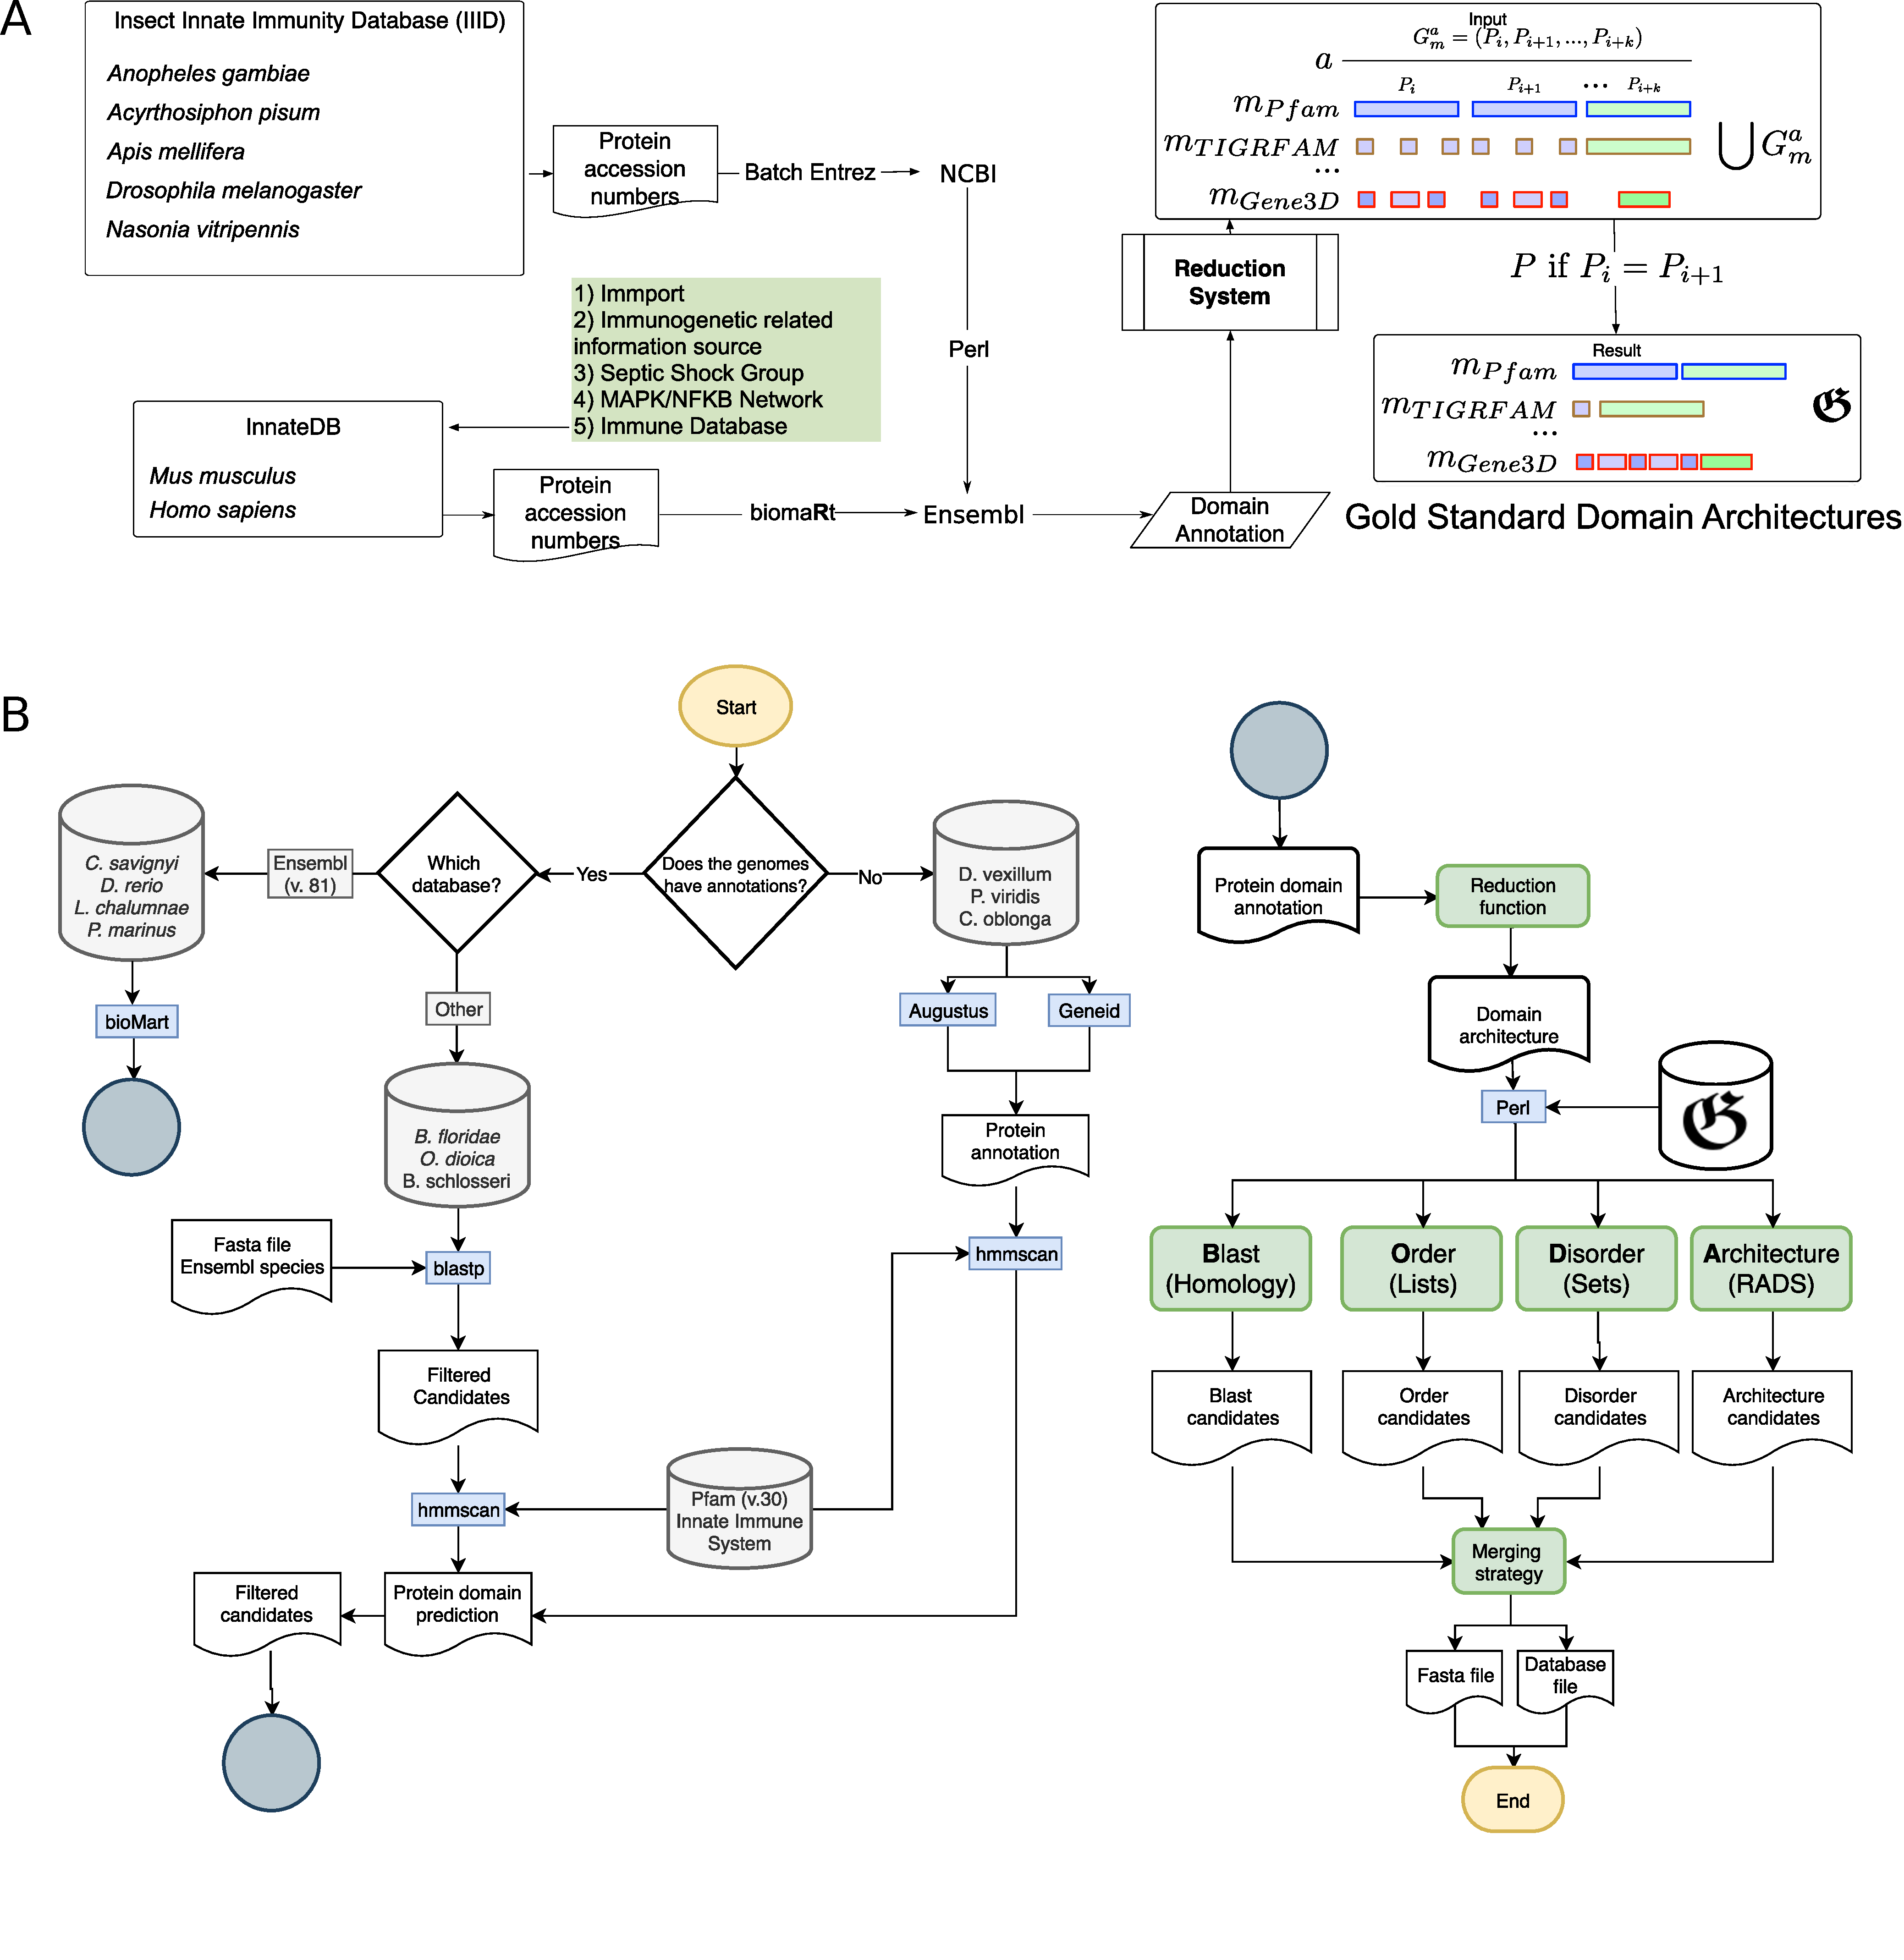
\includegraphics[scale=0.15]{figures/completeALLWorkflow3}
\caption{\textbf{A.} Workflow to generate $\boldsymbol{\mathfrak{G}}$. Innate 
immune system databases were used to obtain the accession numbers of the 
related proteins. Next, domain annotation was accesed throught \texttt{biomaRt} 
from \texttt{Ensembl} (v.81). Post processing include reduction of the 
consecutive repetitions of protein domains and finally, the definition of 
$\boldsymbol{\mathfrak{G}}$. \textbf{B.} Methodological steps to obtain innate 
immune system candidates based on $\boldsymbol{\mathfrak{G}}$ definition. 
Used programs from software packages (HHMer and blast) and in-house 
\texttt{Perl} scripts have been highlighted in blue. In green are indicated the 
\texttt{Perl} scripts that perform the reduction function and each step of 
comparison of architectures (A, B, D, O).}  
\label{workflow_golden}
\end{center}
\end{figure}

%\begin{figure}[htbp]
%\begin{center}
%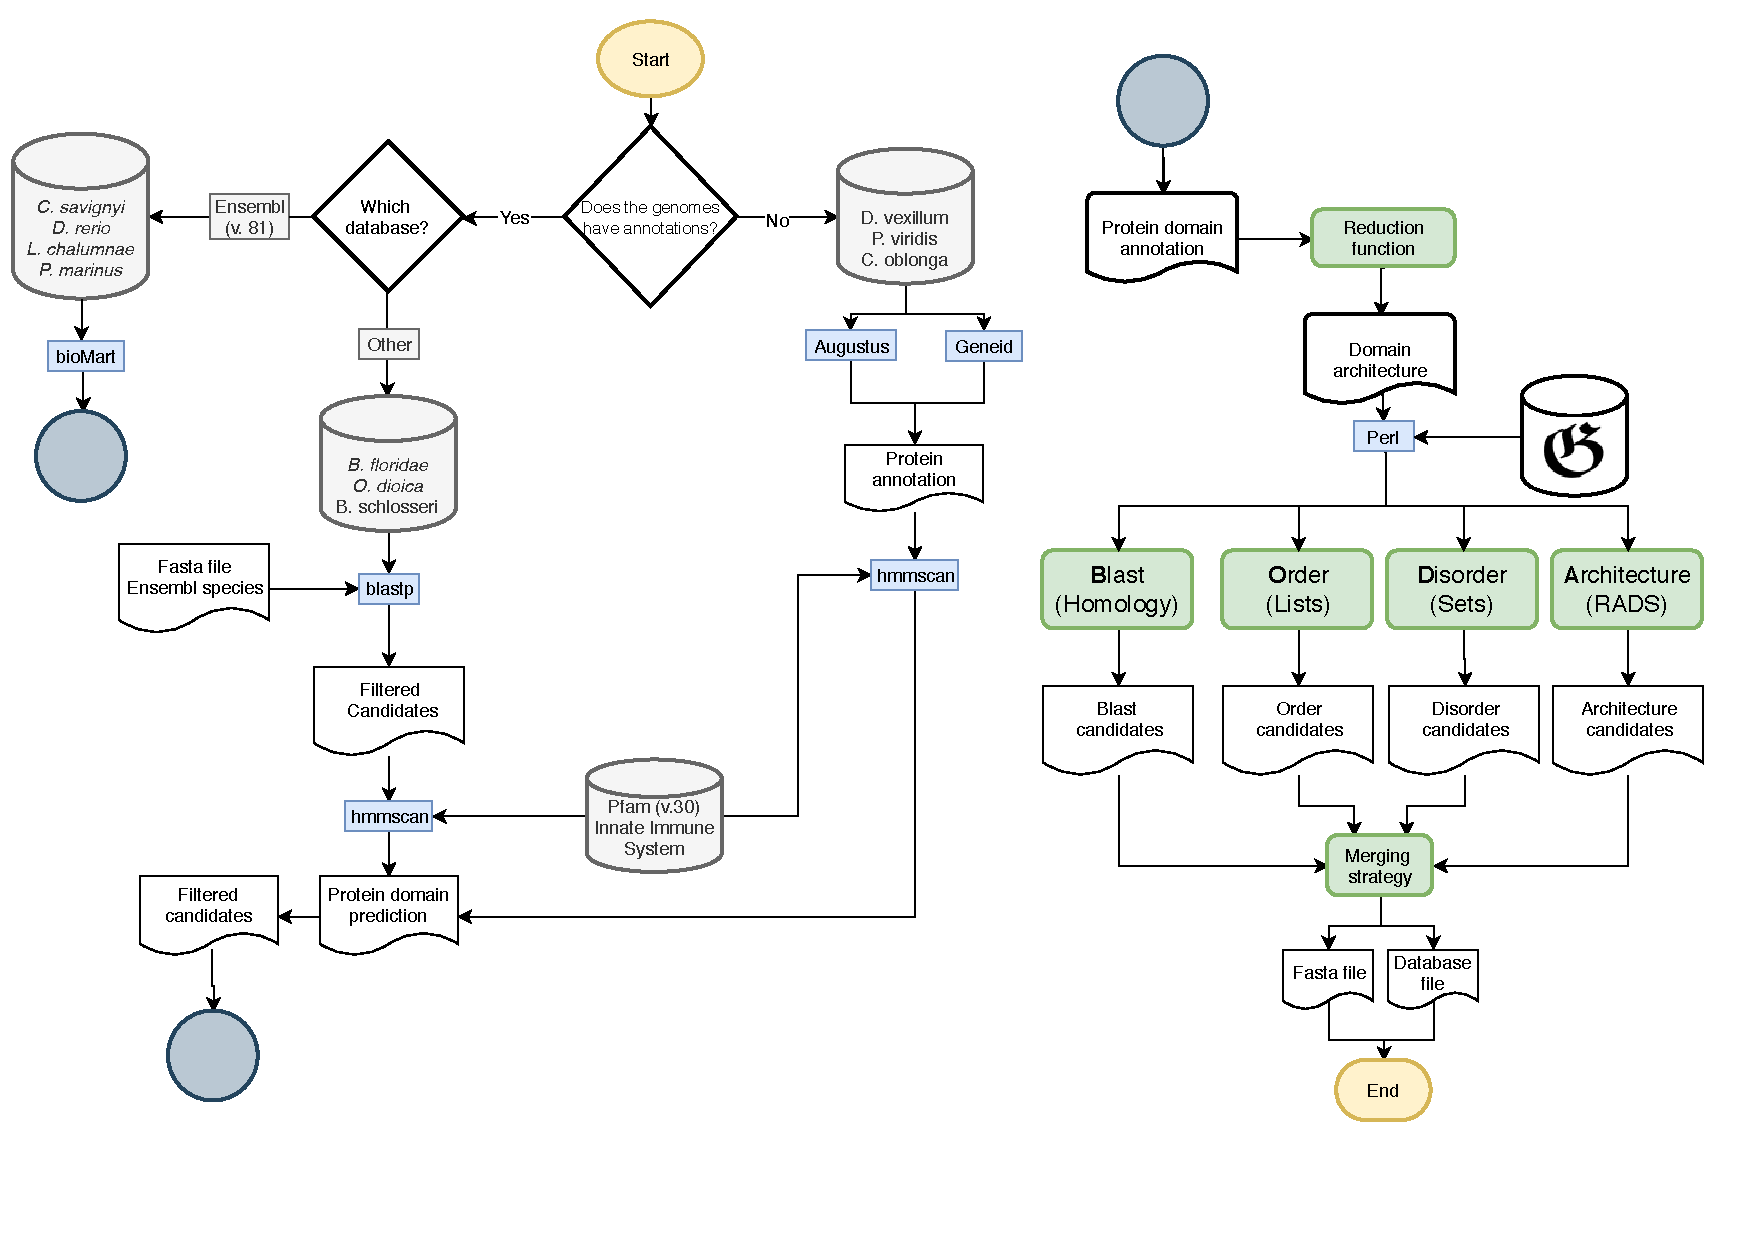
\includegraphics[scale=0.45]{figures/workflowComplete}
%\caption{Methodological steps to obtain innate immune system candidates. 
%Have been highlighted in blue the programs used in this pipeline. In green, 
%those scripts in \texttt{Perl} that performed the reduction function and each 
%of the architecture comparison considered in this study.}
%\label{workflow_domains}
%\end{center}
%\end{figure}

%\begin{figure}[htbp]
%\begin{center}
%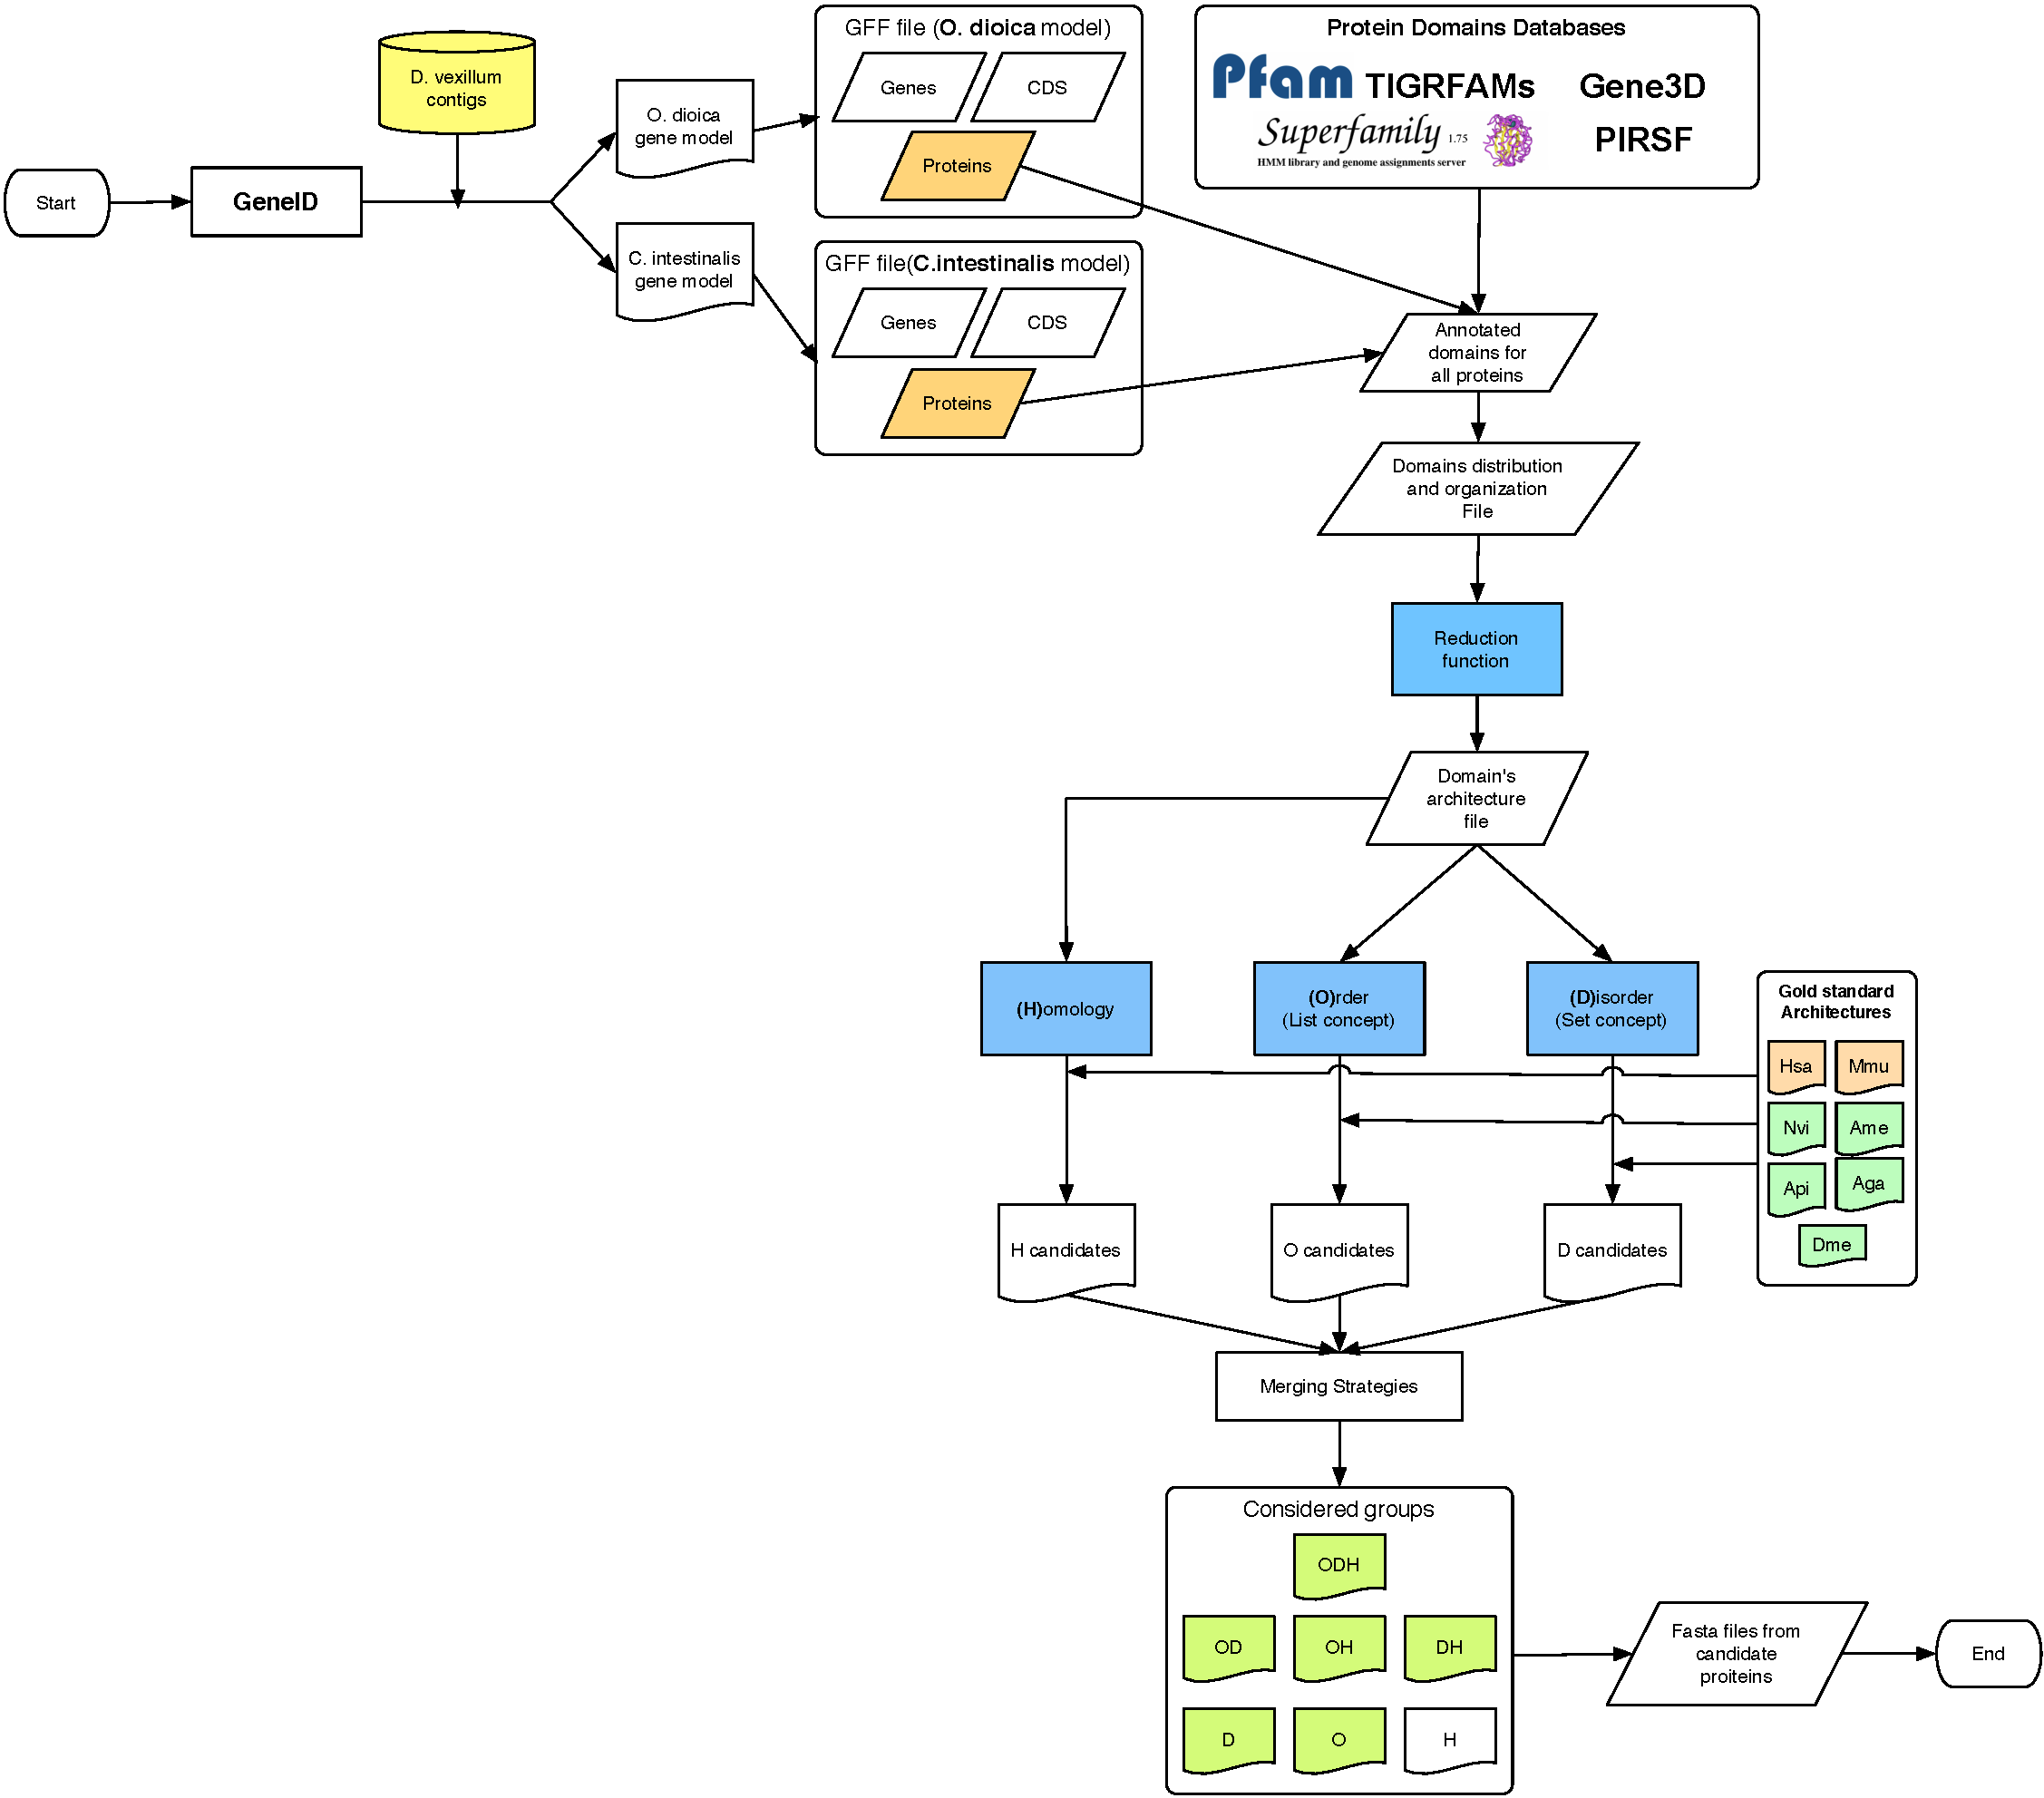
\includegraphics[scale=0.3]{figures/workflow_2_dvex}
%\caption{Designed workflow to annotate genes \textit{de novo} in \textit{D. 
%vexillum} genome, and subsequently obtain the architecture distributions 
%according to \textbf{O}rdered, \textbf{D}isorder and \textbf{B}last strategy.}
%\label{workflow_domains_dvex}
%\end{center}
%\end{figure}

%\begin{figure}[htbp]
%\begin{center}
%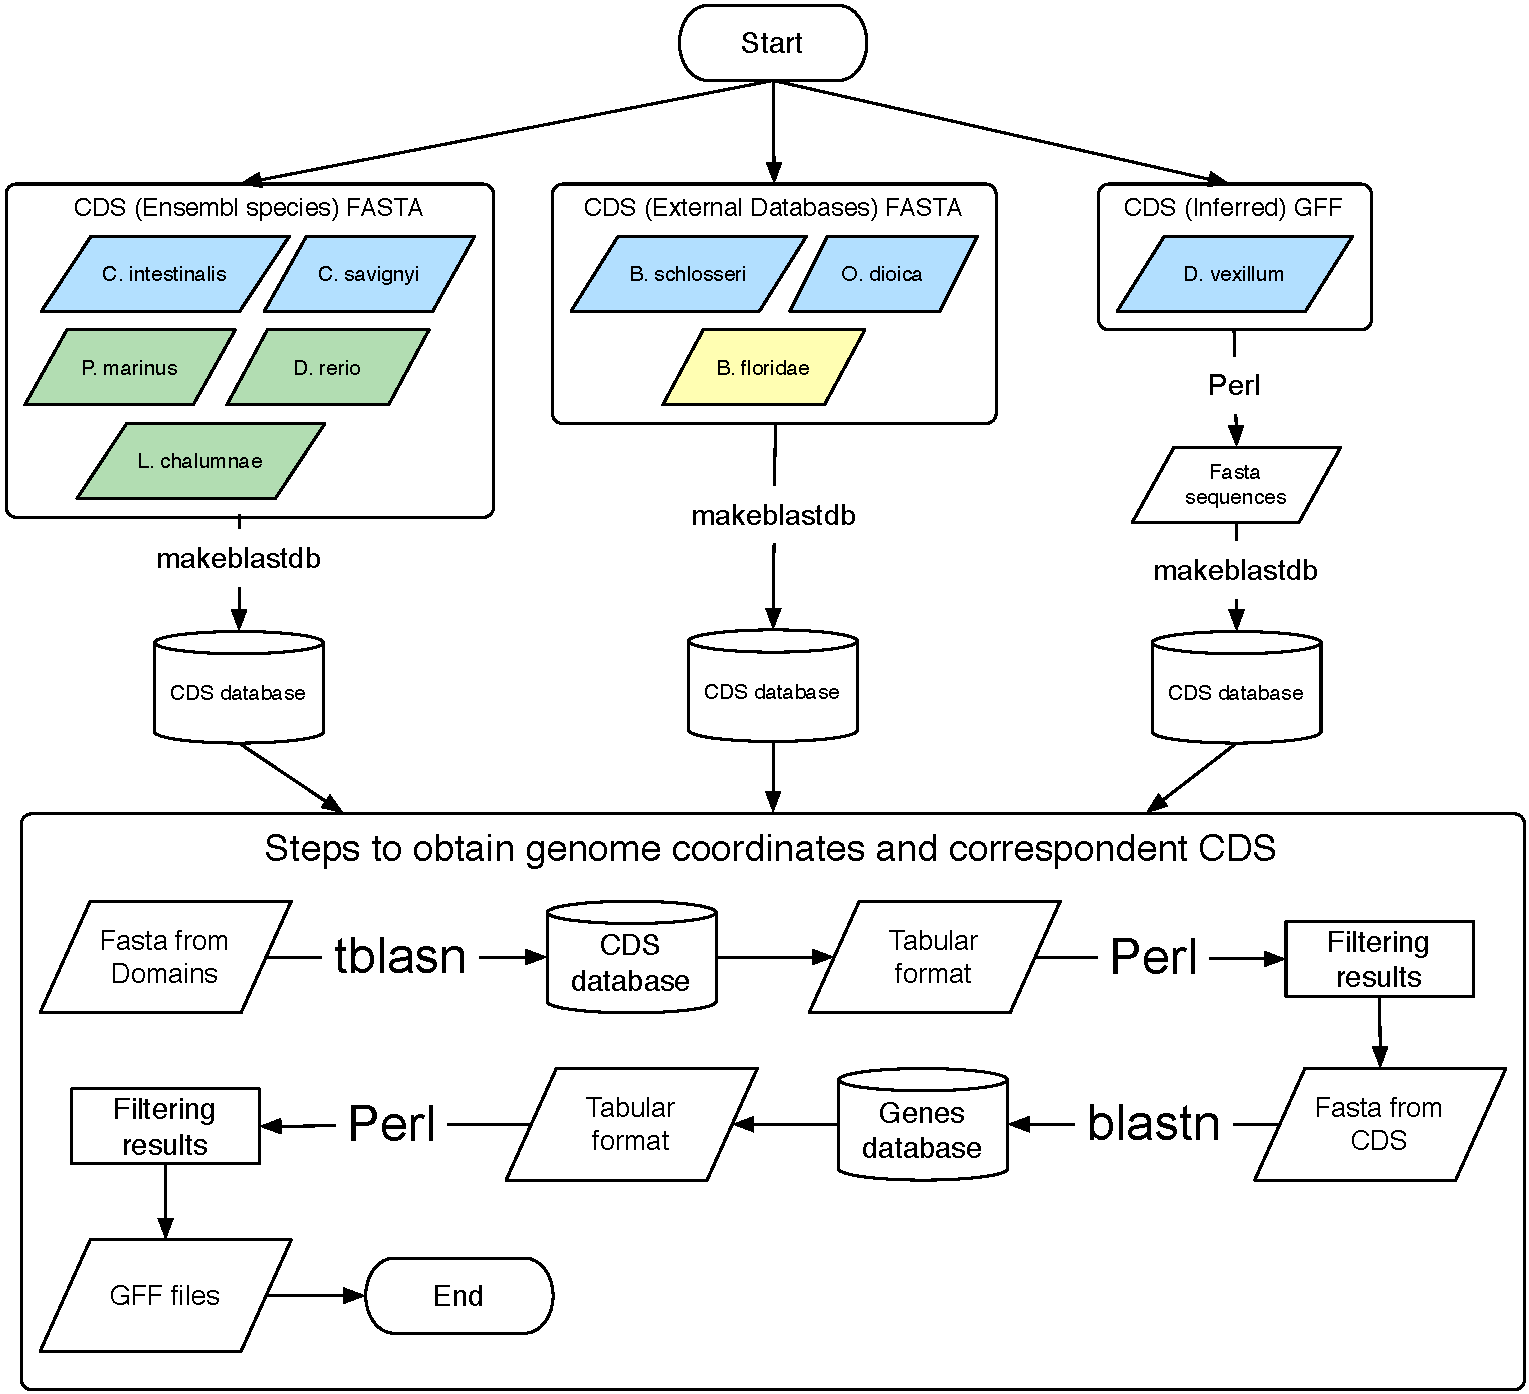
\includegraphics[scale=0.3]{figures/prot2cds}
%\caption{Designed workflow to annotate genes \textit{de novo} in \textit{D. 
%vexillum} genome, and subsequently obtain the architecture distributions 
%according to \textbf{O}rdered, \textbf{D}isorder and \textbf{B}last strategy.}
%\label{proteindomains2cds}
%\end{center}
%\end{figure}

\subsection*{Orthology detection between candidate innate immune system 
proteins}
In order to detect orthologous groups among innate immune system candidates, 
proteins that reported the same architecture relationships respect to the gold 
standard proteins, were compared with \texttt{ProteinOrtho} 
(v.5.16) \cite{Lechner2011}, as follows:

%In order to detect orthology relationships among immune system candidates, CDS 
%sequences that correspond to the protein domains related to the immune system 
%were compared. With the identification of the orthology sets, the number of 
%accession that have been associated to the correspondent mRNAs and with the 
%associated sequence, CDSs for each protein was retrieved, thereby a strategy 
%with the CDS's fragments where applied running \texttt{ProteinOrtho} v.5.16. 
%\cite{Lechner2011} using the \texttt{Poff} extension of synteny, as follows:
\TODO{Change protein ortho parameters according to the discussion about groups 
and orthology relationships.}
\begin{lstlisting}[language=bash, breaklines=true]
#Step 1:
proteinortho5.pl -synteny -dups=3 -verbose -cpus=8 -clean 
-keep -project=<name-project> -step=1 -temp=${temp-directory} -p=blastn 
<fasta file>
#Step 2:
proteinortho5.pl -synteny -dups=3 -graph -cpus=8 -verbose -clean 
-step=2 -project={name-project} -keep -startat=${step} -stopat=4 -p=blastn 
<fasta file>
#Step 3:
proteinortho5.pl -synteny -dups=3 -graph -cpus=16 -verbose -clean -step=3 
-keep -project=<name-project> -p=blastn <fasta file>
\end{lstlisting}

% Here this referenced some orthology groups based on different species 
%comparisons, (re-run?)
%Complete comparisons were performed independently for each domain annotation 
%source $m$. At the same time, different set of comparisons were used to obtain 
%orthology groups between: Tunicates + Cephalochordata (\texttt{B. floridae}); 
%Tunicates + Vertebrata (\textit{P. marinus}) and Vertebrates (\textit{P. 
%marinus}) + Tunicates + Cephalochordata (\texttt{B. floridae}). Output files 
%were analyzed with \texttt{Perl} scripts to get the orthology relationships 
%between orthologous CDS sequences. At the end, with these methodology was 
%possible to obtain orthology groups of genes, that further were subject to 
%built matrices to calculate gain and losses of domains. 

\TODO{
\subsection*{Gain and losses of domains}

Derived from our orthologous relationships we obtained raw and family-specific 
presence/absence matrices of domains. The combined presence/absence matrices 
were subjected to analysis with Count \cite{csuros2010}, reconstructing the 
family history by Dollo parsimony. The phylogenetic distribution of this species 
were obtained from [71] for tunicates, and for the other organisms from Ensembl 
compara [72].
}
\section*{Results}

\subsection*{Global distribution of domains}

\iffalse

Specie Genes Transcripts Proteins
hsa 7043 35136 35136
mmu 1803 5179 5179
#Insects
acpi 81 81 81
anga 329 333 333
apme 106 106 106
drme 202 242 242
navi 368 368 368

\fi

A total of $8846$ genes associated with the innate immune system were recovered 
from \texttt{InnateDB}, of which $7043$ and $1803$ belong to human and mouse 
respectively. After interfaced these records with Ensembl Genome Browser a total 
of $35136$ and $5179$ proteins were identified. Next, to integrate domains 
from the source \texttt{Insect Innate Immunity Database} (IIID) a total of 
$1312$ proteins were recovered distributed as follows: \textsl{N. vitripennis} 
$393$ ($368$), \textsl{A. mellifera} $170$($106$), \textsl{D. melanogaster} 
$298$($242$), \textsl{A. gambiae} $366$ ($333$) and \textsl{A. pisum} 
$85$($81$), the number in parenthesis corresponds to the \textsl{bone fide} 
annotation in \texttt{Ensembl}. Finally the domain structure was traced back 
with \texttt{Biomart} in \texttt{Ensembl}. With the final set of domains we 
built the \textsl{gold standard} set $\boldsymbol{\mathfrak{G}}$ as described 
in Additional File 1. 

\subsection*{\textbf{ABDO} strategy comparisons of domains} \label{subODB}

The distribution of genes and proteins that belong from \textsl{gold standard set} 
$\boldsymbol{\mathfrak{G}}$ is shown on Additional File 1: Table 1, where most of
the current innate inmune system proteins belongs from human ($84.74$\%) and mouse ($12.51$\%).
In order to compare $\boldsymbol{\mathfrak{G}}$ to the query species, the previously explained 
\textbf{ABDO} strategies were applied. As shown in Table \ref{table:distribution_prot}, exists 
$4$ different groups of species: those ones that have been annotated in \texttt{Ensembl} as: 
\textit{C\. robusta}, \textit{C.\ savignyi}, \textit{P.\ marinus}, \textit{D.\ rerio} 
and \textit{L.\ chalumnae}. Next, those ones that have gene and protein annotations but,
in an independent databases and without the prediction of domains, as: \textit{B.\ floridae},
\textit{B.\ schlosseri} and \textit{O.\ dioica}. The other third one is composed by those 
genomes that have a \textsl{de novo} assembly, like: \textit{D.\ vexillum}, 
\textit{C.\ oblonga} and \textit{P.\ viridis}, where does not exists reported predictions 
of genes or proteins, then this prediction were performed as described in Methods and 
Materials with the \texttt{GeneId} program using the previously constructed 
gene models from \textit{C.\ robusta} and \textit{O.\ dioica}\footnote{For 
those genomes, in Table \ref{table:distribution_prot} are referenced as 
\textsl{Ciro} and \textsl{Oidi} in parenthesis, respectively} and with 
\texttt{AUGUSTUS} using transcriptome data. Finally, the last group is composed 
by the outgroup species from hemichordates: \textit{S.\ kowalevskii} and
from echinoderms: \textit{P.\ miniata} and \textit{S.\ purpuratus}, where the \textbf{ABDO} 
predictions have been calculated with the automated pipeline \TODO{NAME\_PIPELINE} generated
in this study.

Table \ref{table:distribution_prot} summarizes the final innate immune system 
candidates, based on homology architecture strategies (\textbf{ABDO}), which 
have been applied independently. The final number of immune system set results 
of the merging of all the candidates obtained from the applied strategies, 
except for the candidates that have been detected only by the \textbf{B} 
strategy. The main reason is that comparison does not represent an 
pure architecture relation, because the complete sequence is used in the 
pairwise alignment, this method has been frequently used to detect homologs 
in distant or related species, according to the design of the homology strategy 
based on the \texttt{blastp} parameters \TODO{CITE}. When it was applied, 
always the B strategy reported higher frequencies of protein candidates in 
comparison to the O or D strategies; and those results are more similar to the 
A strategy, which does not have a previous reduction step. 

Then taking all into account, Table \ref{table:distribution_prot} shows the 
highest distribution from annotated immune system proteins in vertebrates 
(median = $63.49$\% $\pm 4.87$, n=3), in comparison to tunicates 
(median = $31.88$\% $\pm 22.27$, n=12), cephalochordates ($43.14$\%, n=1), and the
outgroup composed by hemichordates ($42.89$\%, n=1) and echinoderms 
(median = $45.15$\% $\pm 11.56$, n=2). High standard deviation in tunicates are 
a consequence of the inclusion of the new draft genomes (from \textit{C.\ oblonga} 
and \textit{P.\ viridis}), where the prediction of genes was \textsl{de novo} 
by \texttt{GeneId}. In this context, only considering the tunicates genomes that 
had a previous annotation, the estimated values changed: (median =$40.21$\% $\pm 13.37$, n=8).

\begin{sidewaystable}
\small
\centering
\begin{tabular}{p{3.2cm}p{2cm}p{2cm}p{2cm}p{2cm}p{2cm}p{2cm}p{2.7cm}p{2.6cm}}
\toprule
\textbf{Specie}&\textbf{Annotated Genes}&\textbf{Annotated 
Proteins}&\textbf{Annotated Prot. with Pfam domains}&\textbf{Orderded 
Prot}&\textbf{Disorder Prot}&\textbf{Blast 
Prot}&\textbf{Architecture}&\textbf{Total Prot IS} \\ 
\midrule \\
\textsl{P. miniata}&    
$30399$&$30399$&$20192$($66.42$)&$1936$($6.37$)&$2527$($8.31$)&$11577$($38.08$)&
$15707$($51.67$)&$16210$($53.32$)\\
\textsl{S. purpuratus}& 
$33663$&$35786$&$23640$($66.06$)&$3248$($9.08$)&$4218$($11.79$)&$15420$($43.09$)
&$10706$($29.92$)&$13230$($36.97$)\\
\textsl{S. kowalevskii}&        
$32367$&$22111$&$14888$($67.33$)&$1973$($8.92$)&$2571$($11.63$)&$9737$($44.04$)&
$8280$($37.45$)&$9483$($42.89$)\\
\midrule
\textsl{B. floridae}&   $50817$&$50817$&$25430$($50.04$)&$5499$($10.82$)&$7352$($14.47$)&$21767$($
42.83$)&$5496$($10.82$)&$21920$($43.14$)\\
\textsl{O. dioica}&$17212$&$17212$&$5709$($33.17$)&$1342$($7.80$)&$1633$($9.49$)&$4577$($26.5
9$)&$4760$($27.66$)&$5065$($29.43$)\\
\textsl{M. occidentalis}&       
$30639$&$33023$&$13050$($39.52$)&$1195$($3.62$)&$1486$($4.50$)&$7170$($21.71$)&$
11152$($33.77$)&$11341$($34.34$)\\
\textsl{M. oculata}&    
$15313$&$16616$&$9985$($60.09$)&$1336$($8.04$)&$1689$($10.16$)&$6615$($39.81$)&$
8355$($50.28$)&$8620$($51.88$)\\
\textsl{B. schlosseri}& $46519$&$46519$&$8709$($18.72$)&$1790$($3.85$)&$2520$($5.42$)&$6148$($13.2
2$)&$6760$($14.53$)&$7316$($15.73$)\\
\textsl{B. leachii }&   
$15839$&$15839$&$9833$($62.08$)&$1271$($8.02$)&$1698$($10.72$)&$6243$($39.42$)&$
8032$($50.71$)&$8369$($52.84$)\\
\textsl{C. robusta} 
&$17153$&$17302$&$8994$($51.98$)&$1371$($7.92$)&$1584$($9.15$)&$6005$($34.71$)&$
4188$($24.21$)&$4958$($28.66$)\\
\textsl{C. savignyi}&
$12172$&$20157$&$14016$($84.84$)&$2087$($10.35$)&$3273$($16.24$)&$10049$($
49.85$)&$10074$($49.98$)&$10923$($54.19$)\\
\textsl{P. viridis} (Ciro)&     
$6077$&$2221773$&$2806$($0.13$)&$56$($0.00$)&$65$($0.00$)&$12724$($0.57$)&$1896$
($0.09$)&$1865$($0.08$)\\
\textsl{P. viridis} (Oidi)&     
$3025$&$1811030$&$2110$($0.12$)&$60$($0.00$)&$72$($0.00$)&$10329$($0.57$)&$1352$
($0.07$)&$1319$($0.07$)\\
\textsl{D. vexillum}&
$26546$&$72326$&$36075$($49.88$)&$2920$($4.04$)&$4136$($5.72$)&$16889$($23.35$)&
$26400$($36.50$)&$27349$($37.81$)\\
\textsl{C. oblonga} (Ciro)&     
$19507$&$1174882$&$4032$($0.34$)&$120$($0.01$)&$161$($0.01$)&$4070$($0.35$)&$282
8$($0.24$)&$2810$($0.24$)\\
\textsl{C. oblonga} (Oidi)&     
$4832$&$950470$&$2856$($0.30$)&$125$($0.01$)&$164$($0.02$)&$8746$($0.92$)&$1957$
($0.21$)&$1939$($0.20$)\\
\midrule
\textsl{P.\ marinus}
&$13114$&$11444$&$9214$($80.51$)&$1650$($14.42$)&$2143$($18.73$)&$6227$($5
4.41$)&$6023$($52.63$)&$7008$($61.24$)\\
\textsl{D.\ rerio}
&$31953$&$44489$&$38629$($86.83$)&$11762$($26.44$)&$13654$($30.69$)&$28031$
($63.01$)&$20992$($47.18$)&$31395$($70.57$)\\
\textsl{L.\ chalumnae}
&$22628$&$23603$&$19509$($82.65$)&$4461$($18.90$)&$5824$($24.67$)&$9127$($3
8.67$)&$10765$($45.61$)&$14986$($63.49$)\\
\bottomrule
\end{tabular}
\caption{Final distribution of annotated genes and found candidate Immune 
system proteins. The percentage in relation of the total of reported proteins 
is in parenthesis.}
\label{table:distribution_prot}
\end{sidewaystable}

Due the application of ABDO strategies was independently, it is possible to 
identify the relationships between the query species and the 
$\boldsymbol{\mathfrak{G}}$ species in the final set of immune system 
candidates through an architecture relationships. As shown in Figure 
\ref{fig:FrecEstrat}A different combinations of possible architecture 
comparison strategies have been merged to four different sets, according to the 
number of (ABDO) strategies that reported a successfully architecture 
comparisons. Here, $1 = (A, D)$; $2 = (AB, AD, BD, DO)$; $3 = (ABD, ADO, BDO)$ 
and $4 = (ABDO)$; that is $10$ from $15$ possible combinations, because $(AO, 
BO)$ always map to $(ADO, BDO)$, due $D \subseteq O$ and additionally, $B$ has 
not been considered at all. This distribution of relationships against 
$\boldsymbol{\mathfrak{G}}$ set shows a highest number of proteins that have 
been detected as immune system candidates by only $1$ architecture strategy. 
Additionaly, the number of candidates that have been detected with all the 
strategies (set $4$) reported frequencies $\leq 5000$ proteins on the subject 
species, reporting the highest distribution on the specie \textit{D.\ rerio}, 
this group represents, along all the comparisons, the most conserved set of 
immune proteins respect to the defined $\boldsymbol{\mathfrak{G}}$. Considering 
in overall the immune system proteins along all the studied species, it is 
possible to identify the proportion of shared innate immune system proteins 
respecto to $\boldsymbol{\mathfrak{G}}$ (Figure \ref{fig:FrecEstrat}B). Mainly 
those relationships have been detected with human and mouse proteins, as 
described earlier, those protein candidates are the most frequent proteins in 
$\boldsymbol{\mathfrak{G}}$.

\begin{figure}[ht!]
\centering
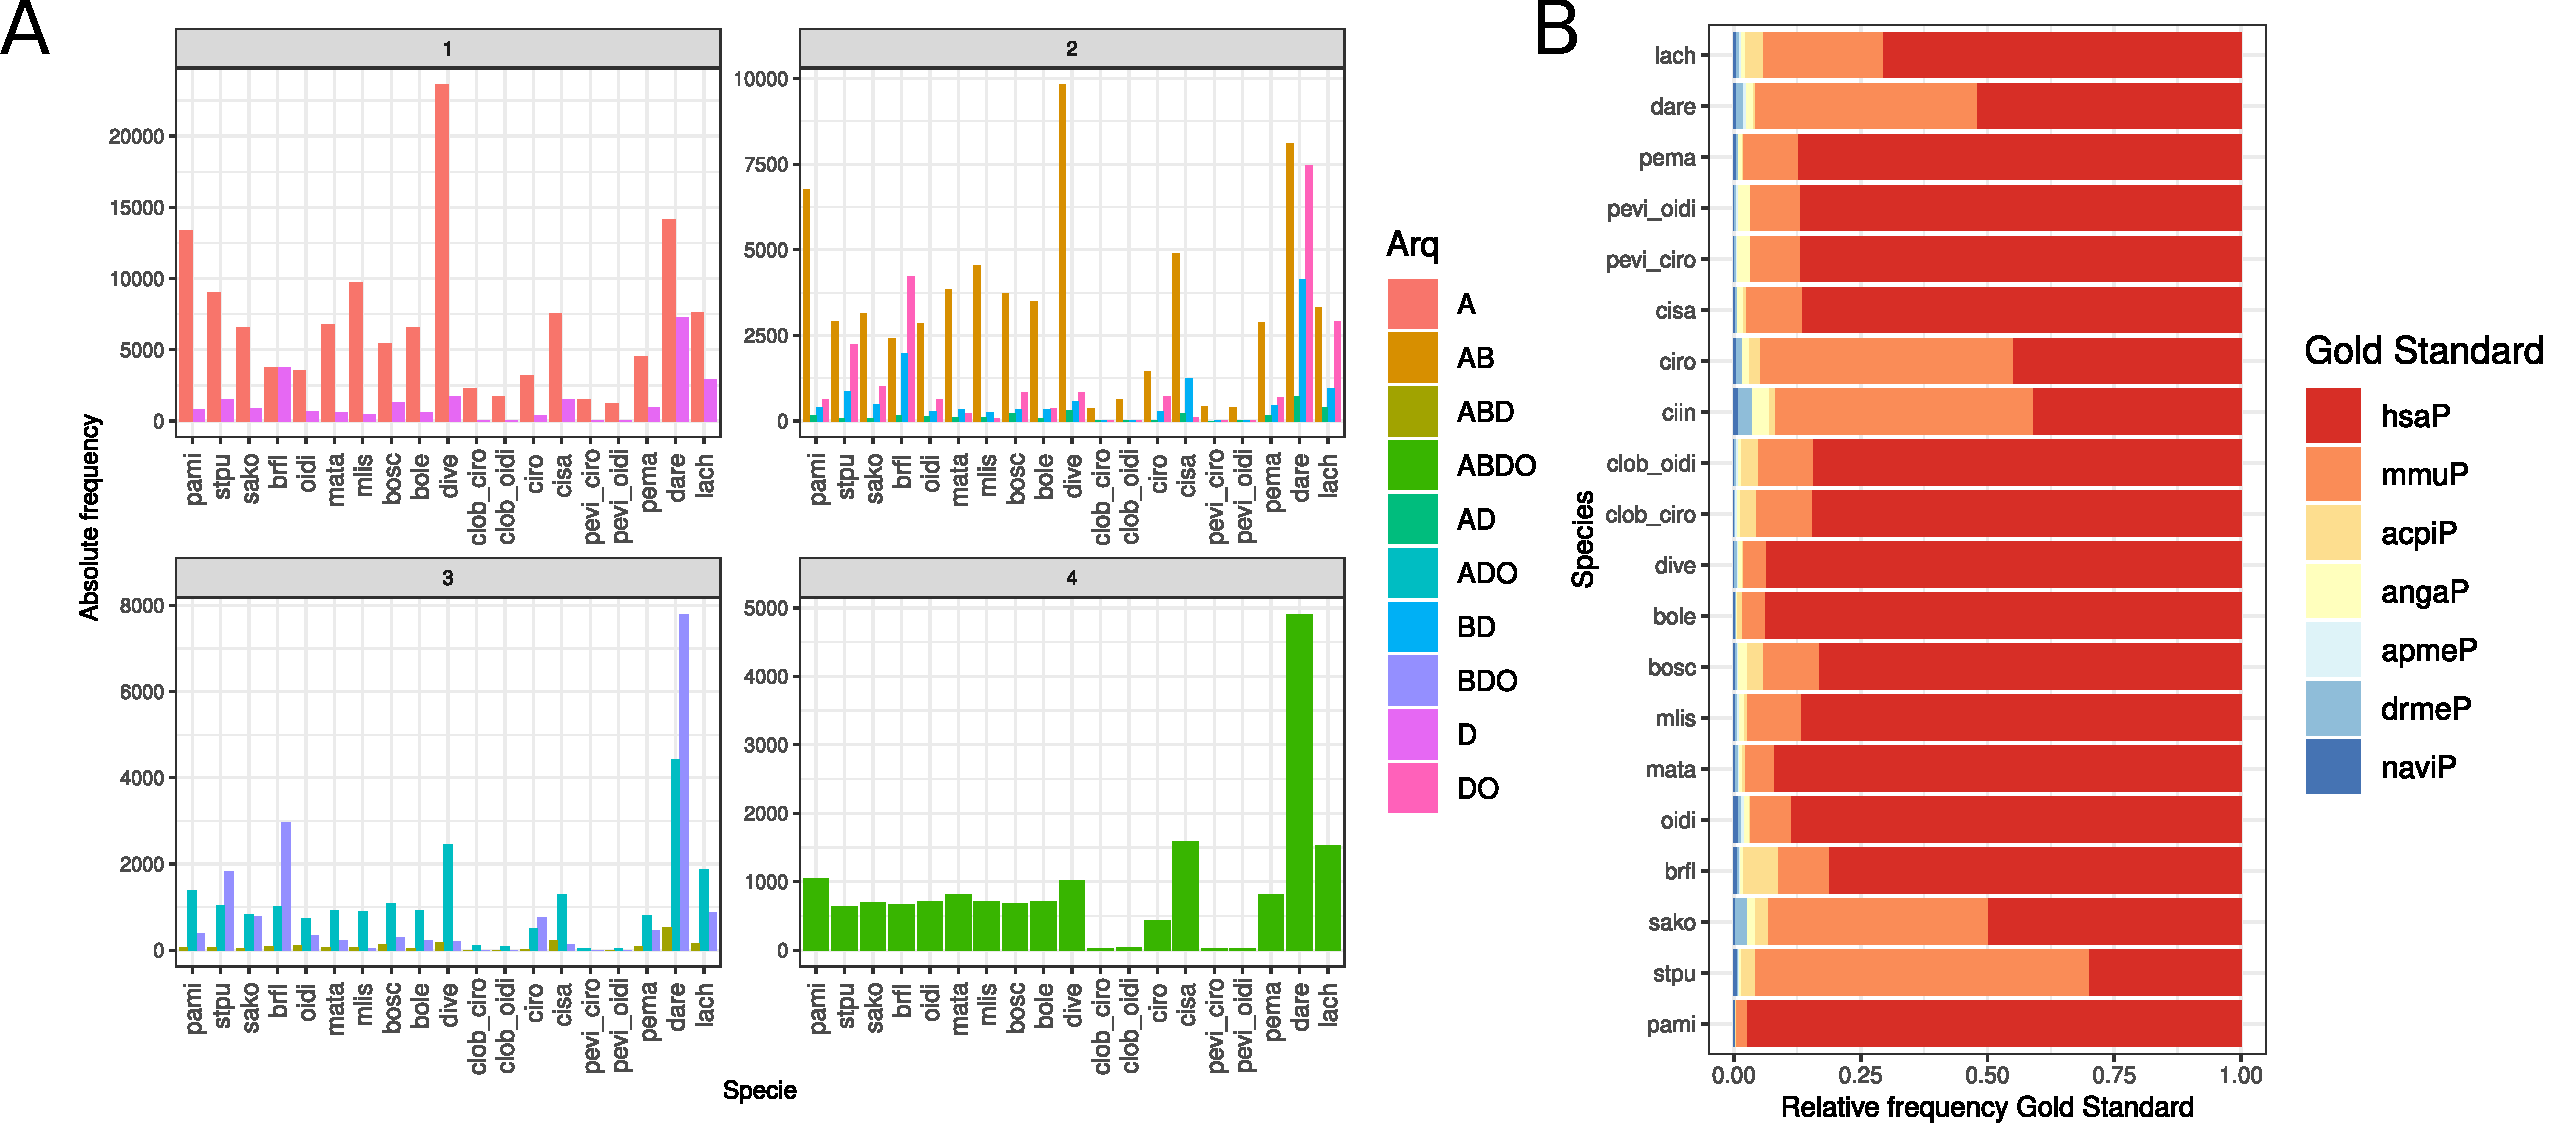
\includegraphics[scale=0.43]{figures/unitedComparedGOLD}%
\caption{\textbf{A.}Frequency of detected proteins with defined architecture
comparison strategies classified according to the number of possible combinations of 
architecture strategies (described in more detail in main text), 
against $\boldsymbol{\mathfrak{G}}$. \textbf{B.} Mean shared proportion homology 
architecture against gold standard species. \textsf{naviP=}\textit{N.\ 
vitripennis}, \textsf{apmeP=}\textit{A.\ mellifera}, \textsf{drmeP=}\textit{D.\ 
melanogaster}, \textsf{angaP=}\textit{A.\ gambiae} and 
\textsf{acpiP=}\textit{A.\ pisum}; and Mammals: \textsf{mmuP=}\textit{M.\ 
musculus} and \textsf{hsaP=}\textit{H.\ sapiens}.}
\label{fig:FrecEstrat}
\end{figure}

%\begin{sidewaysfigure}
%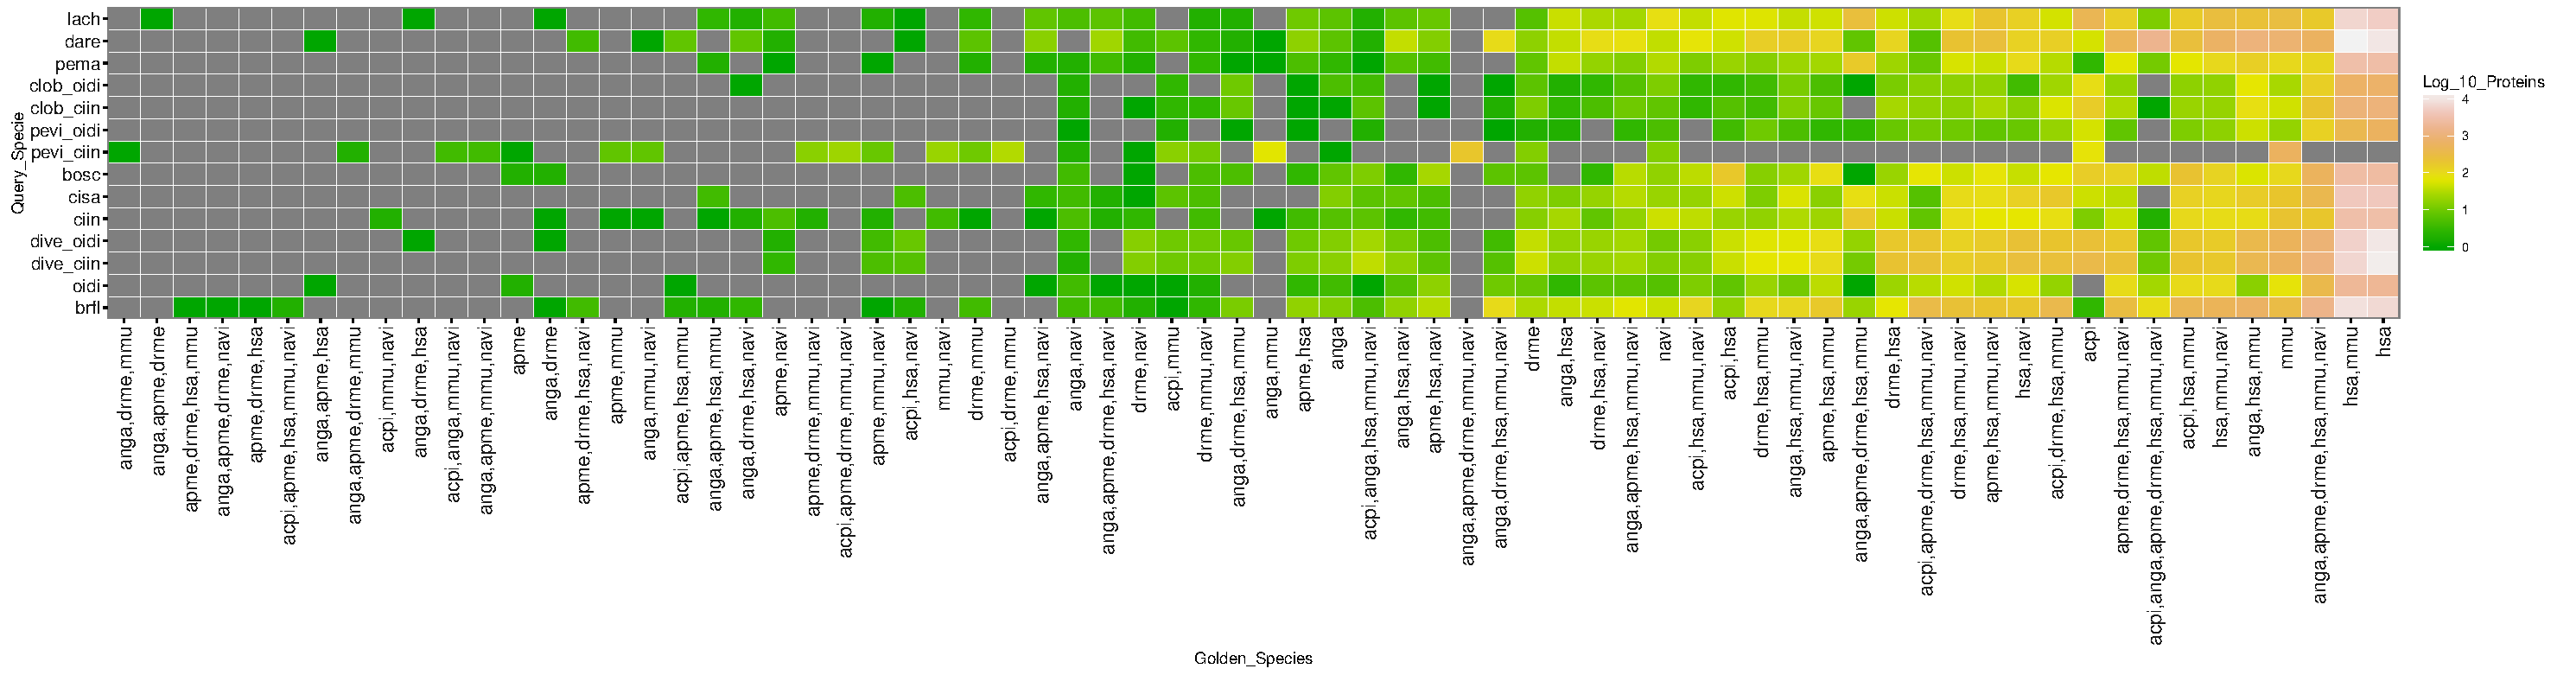
\includegraphics[width=\linewidth,keepaspectratio]{figures/matrix_spe}%
%\caption{Heatmap of the number of proteins identified in the 
%$\boldsymbol{\mathfrak{G}}$ species by at least one of the architecture 
%strategies. The number of proteins have been transformed by $\log_{10} 
%x$. Combinations of species have been obtained according to the final 
%agrupation given by the relationships between Query species and 
%$\boldsymbol{\mathfrak{G}}$ species. This plot have been organized according to 
%the number of final candidates by set of  
%$\boldsymbol{\mathfrak{G}}$ species, left with lower 
%values to the higher ones on the rigth. \textsf{navi=}\textit{N.\ vitripennis}, 
%\textsf{apme=}\textit{A.\ mellifera}, \textsf{drme=}\textit{D.\ melanogaster}, 
%\textsf{anga=}\textit{A.\ gambiae} and \textsf{acpi=}\textit{A.\ pisum}; and 
%Mammals: \textsf{mmu=}\textit{M.\ musculus} and \textsf{hsa=}\textit{H.\ 
%sapiens}.}
%\label{fig:matrix_relations}
%\end{sidewaysfigure}

\subsection*{Relationships between Innate Immune system candidates} 
\label{Orthology}
Once protein candidates were detected by ABDO strategy along studied species, one further step
is the identification of biological relevance of the new detected protein candidates. Applying this clustering 
step was possible identifying the intrinsic relationship between $\boldsymbol{\mathfrak{G}}$ proteins 
and the new identified proteins, based on the protein domain architecture. In this way $4240$ groups
were assigned and in order to identify orthology relationships, \texttt{ProteinOrtho} was applied along
each group. 
The complete distribution of the number of domains inside the identified candidates is show in 
Figure \ref{fig:domainDistr}. Along all the described organisms, grouped by the taxonomical clade, 
it is possible to identify the common distribution of the number of protein domains along all
evaluated proteins. This result is congruent with the idea that protein domain distribution spans
with a Pareto's distribution \cite{}, resulting in a high number of proteins with only one domain and
with a long tail along higher numbers of domains with very low frequency along proteins. Despite 
the similarity of this results along taxonomical clades, distribution from \textsl{B.\ floridae} showed 
higher number of proteins with $2$ domains and similar distribution with Vertebrates on proteins 
with $3$ domains, while Echinoderms, Hemichordates and Tunicates, showed similar density 
distributions in those values. 

At the same time, Table XX shows the most frequent protein architectures and the current 
annotation in \texttt{Pfam} database.  In general the most common proteins domains are shown
in Table XX. For proteins composed by one domain, the most frequent protein domain is a 
Rhodopsin-like receptor (PF00001) for echinoderms, hemichordates and vertebrates, while 
in Cephalochordata was the Cytochrome P450 (PF00067) and for tunicates the Protein Kinase domain 
(PF00069).  At the same time, for heterodomain proteins those ones that are composed by $2$ domains
reported domains involved on recognition as and $3$ domains are more specifically related with immune 
responses. 

%More specificity with more domains?

\begin{figure}[ht!]
\centering
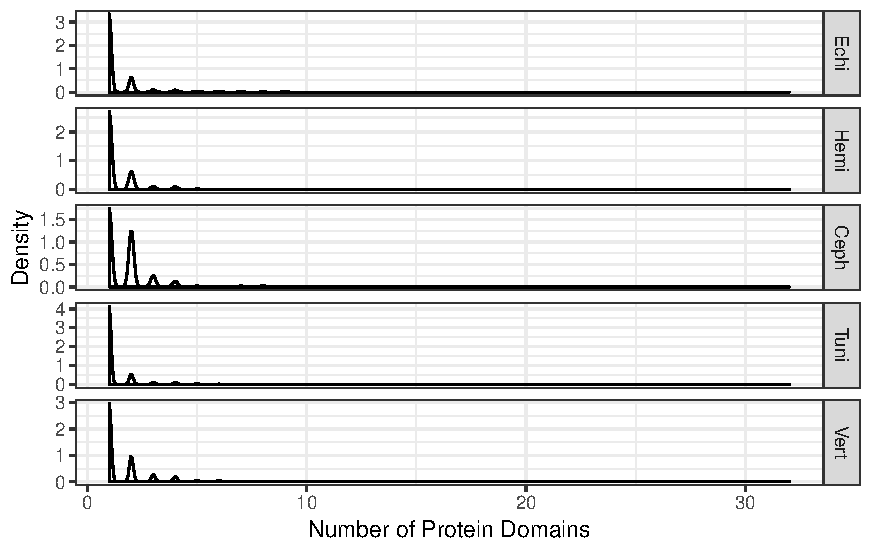
\includegraphics[scale=0.63]{figures/domainDistribution}
\caption{Domain distribution of innate immune system proteins along studied 
bilateria species.\textbf{Echi:} Echinodermata, \textbf{Hemi:} Hemichordata, 
\textbf{Ceph:} Cephalochordata, \textbf{Tuni:} Tunicata and \textbf{Vert:} Vertebrata.}
\label{fig:domainDistr}
\end{figure}

\iffalse
%% TODO: put this info in a table and describe a little bit the annotation.
%1
1 Echi  PF00001        991
2 Hemi  PF00001        438
3 Ceph  PF00067        388
4 Tuni  PF00069       2415
5 Vert  PF00001       1304
%2
1 Echi  PF01825,PF00002   186
2 Hemi  PF02931,PF02932   117
3 Ceph  PF15227,PF00643   313
4 Tuni  PF07707,PF01344   704
5 Vert  PF13281,PF00069  1430
%3
1 Echi  PF00084,PF02494,PF00084    54
2 Hemi  PF00629,PF00057,PF00629    13
3 Ceph  PF12947,PF14670,PF07645   302
4 Tuni  PF12947,PF14670,PF07645   146
5 Vert  PF13927,PF13895,PF13927   366
%4
1 Echi  PF00664,PF00005,PF00664,PF00005   111
2 Hemi  PF00664,PF00005,PF00664,PF00005    46
3 Ceph  PF14670,PF07645,PF00054,PF02210    62
4 Tuni  PF00664,PF00005,PF00664,PF00005   200
5 Vert  PF14670,PF07645,PF00054,PF02210   110
%5
1 Echi  PF07679,PF00041,PF07679,PF00041,PF07679    33
2 Hemi  PF07679,PF00041,PF07679,PF00041,PF07679    11
3 Ceph  PF00651,PF13912,PF12874,PF13912,PF12874    15
4 Ceph  PF13855,PF00791,PF10461,PF00791,PF00531    15
5 Tuni  PF03104,PF15735,PF03104,PF00136,PF14260   188
6 Vert  PF00651,PF13912,PF12874,PF13912,PF12874   118
%6
1 Echi  PF00246,PF13620,PF00246,PF13620,PF00246,PF13620    12
2 Echi  PF00270,PF00271,PF02889,PF00270,PF00271,PF02889    12
3 Hemi  PF00246,PF13620,PF00246,PF13620,PF00246,PF13620     4
4 Ceph  PF00246,PF13620,PF00246,PF13620,PF00246,PF13620    20
5 Tuni  PF00111,PF01799,PF00941,PF03450,PF01315,PF02738    33
6 Vert  PF13912,PF00096,PF13912,PF00096,PF13912,PF00096    35
%7
1 Echi  PF00008,PF07645,PF00008,PF07645,PF00008,PF07645,PF00008    30
2 Hemi  PF00008,PF07645,PF00008,PF07645,PF00008,PF07645,PF00008     6
3 Ceph  PF00008,PF07645,PF00008,PF07645,PF00008,PF07645,PF00008    21
4 Tuni  PF00008,PF07645,PF00008,PF07645,PF00008,PF07645,PF00008    63
5 Vert  PF07645,PF00683,PF07645,PF00683,PF07645,PF00683,PF07645     9
6 Vert  PF12661,PF07974,PF12661,PF07974,PF12661,PF00041,PF00147     9
%8
1 Echi  PF00094,PF08742,PF01826,PF00094,PF08742,PF01826,PF00094,PF08742    34
2 Hemi  PF00094,PF08742,PF01826,PF00094,PF08742,PF01826,PF00094,PF08742    35
3 Ceph  PF13912,PF00096,PF13912,PF00096,PF13912,PF00096,PF13912,PF00096    60
4 Tuni  PF00094,PF08742,PF01826,PF00094,PF08742,PF01826,PF00094,PF08742   128
5 Vert  PF13912,PF00096,PF13912,PF00096,PF13912,PF00096,PF13912,PF00096    83
%9
1 Echi  PF00055,PF00053,PF00052,PF00053,PF00052,PF00053,PF06008,PF06009,…     1
2 Tuni  PF13855,PF07679,PF13927,PF07679,PF13927,PF07679,PF13927,PF07679,…    16
3 Vert  PF13855,PF07679,PF13927,PF07679,PF13927,PF07679,PF13927,PF07679,…     7
%10
\fi


%According to the described strategy, the organization of the protein 
%architectures by groups allowed the reduction of the number of comparisons 
%between all the proteins. In this respect, $13146$ sets of similar 
%architectures constituted the database of architectures where all the protein 
%architectures were classified. About $27.54$\% of these groups reported only 
%$1$ member and the $5$ groups that reported the highest 
%number of elements, for instance the archictectures: PF00069 ($9\,326\,916$), 
%hat corresponds to the P-kinase domain; PF00001 ($3\,976\,036$) a 
%hodopsin-like receptors family; PF00147 ($1442401$) fibrinogen alpha chain; 
%PF00059 ($1\,265\,625$) a Lectin C-type domain and PF00067 ($1\,100\,401$) the 
%Cytochrome P450. In addition, Table \ref{tab:domains} describe the protein 
%domains that are overrepresented in the immune system candidate architectures, 
%in this way the most frequent protein domain along all the proteins is the 
%Epidermal grow factor-like domain (PF00008) with a frequency of $4703$ times 
%in 
%the annotation of all the proteins, but also, it is the most frequent domain 
%along all the protein architectures, the same information is described for the 
%$10$ most common domains, asociating their annotation for the GO term. 

\begin{table}[ht!]
\caption{Top ten of most frequent domains found on chordate's immune system 
proteins.}
\begin{center}
\begin{tabular}{p{2.0cm}ccp{4cm}p{3.5cm}}
\toprule
\textbf{Number Architectures}& \textbf{Frecuency} & \textbf{ACC} & 
\textbf{PFAM Annotation} & \textbf{GO term}\\
\midrule
96&1143 & PF00028&Cadherin domain & GO:calcium ion binding; GO:0005509. 
GO:homophilic cell adhesion via plasma membrane adhesion molecules; GO:0007156. 
GO:membrane; GO:0016020\\
422&1183 & PF00096&Zinc finger, C2H2 type & NA \\
185&1385 &PF01391&Collagen triple helix repeat (20 copies) & NA \\
279&1655  &PF00057&Low-density lipoprotein receptor domain class A & 
Ldl\_recept\_a; GO:protein binding; GO:0005515 \\
302&1780 &PF00084&Sushi repeat (SCR repeat) & NA \\
430&2293 & PF13465&Zinc-finger double domain & NA\\
680&3566 &PF07679&Immunoglobulin I-set domain & NA\\
683&3966 &PF07645&Calcium-binding EGF domain & EGF\_CA; GO:calcium ion binding; 
GO:0005509\\
543&4150 &PF00041&Fibronectin type III domain & fn3; GO:protein binding; 
GO:0005515\\
731&4703 &PF00008&EGF-like domain & NA\\
\bottomrule
\end{tabular}
\end{center}
\label{tab:domains}
\end{table}%

\bibliographystyle{abbrvnat}
\bibliography{biblio,otherbibio}

\end{document}
